\documentclass[fontsize=12pt, a4paper,pagesize=auto,toc=listof,twoside,chapterprefix=false,appendixprefix=true,open=right]{scrbook}


% Pacotes usados
% from KOMA
\usepackage{scrhack} % evita warning do lst listings
\usepackage{indentfirst}
\usepackage{needspace}
\usepackage{outlines}
% usa mais interfaces de saída
%  solution for the error “no room for a new \write” (This is a deep magic over TeX)
%\usepackage{morewrites}
%\morewritessetup{allocate=10}

% texto em português
% https://tex.stackexchange.com/questions/13172/detect-which-tex-engine-is-used
\usepackage{iftex}
\ifpdftex
	\typeout{^^J *** PDF MODE ***}
	\usepackage{cmap} % Make PDF files searchable and copyable
	\usepackage[utf8]{inputenc}
	\usepackage{scrwfile}
\fi
\ifluatex
	\typeout{^^J *** LuaLaTeX MODE ***}
\fi

\usepackage[brazilian]{babel}
%\usepackage[T1]{fontenc}

% FONTES USADAS!!!
\usepackage{lmodern}
\usepackage{marvosym}
% bbding tem cross também
\let\Cross\relax
\usepackage{bbding}

\usepackage[dvipsnames]{xcolor}

%%%%%%%%%%%%%%%%%%%% l3packages
% This collection contains implementations for aspects of the LATEX3 kernel, dealing with higher-level ideas such as the Designer Interface
% pacotes i3packages
% frações mais flexíveis
\usepackage{xfrac}
% provides a high-level interface for declaring document commands
\usepackage{xparse}

%%%%%%%%%%%%%%%%%%% FIM l3packages




% to use \currenttime
\usepackage{datetime}

% avoid pdf warning messages from pdflatex
%\pdfminorversion=6



%\usepackage{kpfonts}

% melhor typesetting
\usepackage{microtype}

%
%\usepackage{showframe}
%\usepackage[a4paper]{geometry}
%\usepackage[a4paper,top=2cm,left=2cm,right=2cm,bottom=2cm]{geometry}
%Letra  de início de parágrafo
%\usepackage{lettrine}

% controle melhor dos captions
% Captions e SUB FIGURAS (subcations resolve esse problema melhor)
\usepackage[centerlast,font={small}]{caption}
\setlength{\captionmargin}{1cm}
\usepackage{subcaption}

% usa o H em imagens
%\usepackage{float}

% pacote para gerenciar quotes pequenos e grandes
%tem o comando \enquote
\usepackage[style=brazilian]{csquotes}
% from the manual
\renewcommand*{\mkcitation}[1]{ #1}
% magic for better quotes
%https://latex.org/forum/viewtopic.php?t=5444
\newenvironment*{smallquote}
   {\quote\footnotesize}
   {\endquote}
\SetBlockEnvironment{smallquote}

% Makeindex
% Não está gerando os índices
\usepackage{imakeidx}
\makeindex
\renewcommand{\printindex}{%
  \clearpage
  \phantomsection
  % Comente a linha abaixo se não quiser no sumário:
  % \addcontentsline{toc}{chapter}{Índice Remissivo}
  % Você pode usar \chapter{Índice Remissivo} aqui se quiser com número:
  \markboth{Índice Remissivo}{Índice Remissivo}%
  \input{\jobname.ind}%
}

% vamos usar o biblatex, recomendação
%citestyle=alphabetic,bibstyle=authortitle
\usepackage[ citestyle=authoryear,articlein=false,
style=ext-authoryear-comp
,natbib=true]{biblatex}


% fix "acedido" por algo mais razoável
% fiz "e alli" por "et al."
%\DefineBibliographyStrings{portuguese}{%
%  urlseen={Disponível em}
  %,andothers={et al.},andmore={et al.}
%  }
 % USE and other no campo author para forçar et al.
%\bibliographystyle{plainnat} %without url for book entries
% https://tex.stackexchange.com/questions/445858/changing-reference-style-in-biblatex
%https://tex.stackexchange.com/questions/10682/suppress-in-biblatex
% http://linorg.usp.br/CTAN/macros/latex/contrib/biblatex-contrib/biblatex-ext/biblatex-ext.pdf


%add document elements like a bibliography or an index to the Table of Contents
%\usepackage[nottoc,notlof,notlot]{tocbibind}

\usepackage{graphicx}

% novas keys de trim e valign (usado em vários
% tabelas com imagens
% export permite usar no includegraphics (exporta para ele)
\usepackage[export]{adjustbox}
%\graphicspath{ {./imagens/} }

% The Tkiz packages
\usepackage{pgf,tikz}
\usepackage{mathrsfs}
\usepackage{icomma}


\usepackage{comandos/pgf-pie}
\usepackage[]{tikz-3dplot}
\usetikzlibrary{fadings}

\usetikzlibrary{calc}
\usetikzlibrary{math}
\usetikzlibrary{shadows}
\usetikzlibrary{patterns}
\usetikzlibrary{automata}
\usetikzlibrary{positioning}
\usetikzlibrary{topaths}
\usetikzlibrary{intersections}
\usetikzlibrary{matrix}
\usetikzlibrary{mindmap}

\usetikzlibrary{datavisualization}
\usetikzlibrary{datavisualization.formats.functions}

\usetikzlibrary{arrows}
\usetikzlibrary{arrows.meta}

\usetikzlibrary{shapes}
\usetikzlibrary{shapes.arrows}
\usetikzlibrary{shapes.symbols}
\usetikzlibrary{shapes.geometric}

\usetikzlibrary{decorations}
\usetikzlibrary{decorations.shapes}
\usetikzlibrary{decorations.pathmorphing}
\usetikzlibrary{decorations.text}
\usepgflibrary{decorations.pathreplacing}
\usepgflibrary{decorations.markings}
\usepgflibrary{decorations.footprints}
\usepgflibrary{decorations.fractals}

\usepackage{pgfplots}
\usepackage{pgfplotstable}
\pgfplotsset{compat=1.14}





%\usetikzlibrary{3d}



% esse parametro evita
% que o texto seja separado da imagem
% e facilita (muito) tratar o tamanho
\usepackage[inkscapelatex=false]{svg}

%controla onde ficam os floats
% não queremos que pulem uma entrada
% usa o commando \FloatBarrier
\usepackage[section]{placeins}

% para addlinespace e toprule
\usepackage{array}
\usepackage{booktabs}
\usepackage{multirow}
\usepackage{multicol}

% permite novos tipos de colunas em Tabelas
% e ainda uma definição dinâmica
\usepackage{tabularx}
\newcolumntype{T}{>{\centering \arraybackslash}X}

% icons do CC, tem comandos conjuntos
\usepackage{ccicons}
% http://linorg.usp.br/CTAN/fonts/ccicons/ccicons.pdf

%%%%%%%%%%%% ENUMITEM configurado
\usepackage{enumitem}
% queremos menos espaço entre os itens de uma lista
\setlist{nosep}
% criando uma check-box list
\newlist{todolist}{itemize}{2}
\setlist[todolist]{label=$\square$}
% https://tex.stackexchange.com/questions/13463/specifying-bullet-type-when-using-itemize#
% o normal é \circle - e * (muito feio)
%https://texblog.org/2008/10/16/lists-enumerate-itemize-description-and-how-to-change-them/
\renewcommand{\labelitemi}{$\bullet$}
\renewcommand{\labelitemii}{$\circ$}
\renewcommand{\labelitemiii}{$\diamond$}
\renewcommand{\labelitemiv}{$\circle}
% colocando . entre 1a para ficar 1.a
% nos \ref para \labels
% https://tex.stackexchange.com/questions/288407/no-dots-in-the-cross-reference-to-an-item-from-enumerate/288412#288412
% I want dots
\makeatletter
\renewcommand\p@enumii{\theenumi.}
\renewcommand\p@enumiii{\theenumi.\theenumi.}
\makeatother
%%%%%%%%%%%% ENUMITEM END

\usepackage{fancyvrb}

% Controlar a Marca Dagua
%\usepackage{draftwatermark}
%\SetWatermarkText{DRAFT}
%\SetWatermarkScale{5}
%\SetWatermarkColor[gray]{0.90}

\usepackage{amsmath}
\usepackage{amssymb}
\usepackage{amsfonts}
\usepackage{amsthm}
%,exercise}
%\numberwithin{Answer}{chapter}
%\numberwithin{Exercise}{chapter}

% para os exercícios
\usepackage{exsol}
\renewcommand{\exercisename}{Exercício}
\renewcommand{\exercisesname}{Exercícios}
\renewcommand{\solutionname}{Solução}
\renewcommand{\solutionsname}{Soluções}
\renewcommand{\seriesname}{Série}



% minicontent
%https://tex.stackexchange.com/questions/430594/use-minitoc-with-koma-script-scrbook
\usepackage{etoc}
\newcommand{\chaptertoc}[1][Conteúdo]{
	\etocsettocstyle{\addsec*{#1\\\rule{\textwidth}{0.4pt}}}
	{\bigskip}
	\etocsettocdepth{1}
	\localtableofcontents
}


% para caixas legais
\usepackage{tcolorbox}

%para underline que quebra linha
% usar \uline
% o normalem significa manter o \emph como é
% senão ele é alterado para underline
\usepackage[normalem]{ulem}

% Títulos mais legais
%\usepackage[Bjornstrup]{fncychap}
%\usepackage{titlesec}
%\titleformat{\chapter}[hang]{\Huge\bfseries}{\thechapter\hsp\textcolor{gray75}{|}\hsp}{0pt}{\Huge\bfseries}

%Para usar casos de uso, verificar no capítulo
%comandos copiados da rede
\usepackage{comandos/usecases}

% Usando listagens
\usepackage{listings}
\lstset{extendedchars=true,basicstyle=\ttfamily,
		inputencoding=utf8,
            literate=%
            {ã}{{\~{a}}}1
            {á}{{\'{a}}}1
            {â}{{\^{a}}}1
            {à}{{\`{a}}}1
            {é}{{\'{e}}}1
            {è}{{\`{e}}}1
            {ê}{{\^{e}}}1
            {î}{{\^{i}}}1
            {í}{{\'{i}}}1
            {ô}{{\^{o}}}1
            {ó}{{\'{o}}}1
            {õ}{{\~{o}}}1
            {û}{{\^{u}}}1
            {ú}{{\'{u}}}1
            {ç}{{\c{c}}}1
            {Ç}{{\c{C}}}1
            {Ã}{{\~{A}}}1
            {À}{{\`{A}}}1
            {Â}{{\^{A}}}1
            {Á}{{\'{A}}}1
            {É}{{\'{E}}}1
            {Ê}{{\^{E}}}1
            {Î}{{\^{I}}}1
            {Í}{{\'{I}}}1
            {Ó}{{\'{O}}}1
            {Ô}{{\^{O}}}1
            {Õ}{{\~{O}}}1
            {Ú}{{\'{U}}}1
            }

\renewcommand{\lstlistlistingname}{Lista de Programas}
\renewcommand{\lstlistingname}{Lista de Programas}


\usepackage{wrapfig}

\usepackage{etoolbox} 
\usepackage{pdfpages}
\usepackage{setspace}

% para poder usar url
\usepackage{url,xurl}
\usepackage[hidelinks]{hyperref}

% lista de URLS
\newwrite\urllistfile
\immediate\openout\urllistfile=urllist.aux

\let\oldurl\url
\renewcommand{\url}[1]{\myurl{#1}}
\newcommand{\expurl}[2]{\myeurl{#1}{#2}}

\newcommand{\myurl}[1]{%
  \oldurl{#1}%
  \begingroup
    \edef\tempurl{#1}%
    \immediate\write\urllistfile{\noexpand\urllistentry{\tempurl}}%
  \endgroup
}

\newcommand{\myeurl}[2]{%
  \oldurl{#1}%
  \begingroup
    \edef\tempurl{#1}%
    \immediate\write\urllistfile{\noexpand\eurllistentry{\tempurl}{#2}}%
  \endgroup
}

\newcommand{\urllistentry}[1]{\item \oldurl{#1}}
\newcommand{\eurllistentry}[2]{\item \textbf{#2}: \oldurl{#1}}

\newcommand{\listofurls}{%
  \immediate\closeout\urllistfile
  \begin{itemize}
    \input{urllist.aux}
  \end{itemize}
}


% Comandos criados

% star - cannot contain \par (see https://tex.stackexchange.com/questions/1050/whats-the-difference-between-newcommand-and-newcommand)
\newcommand*{\gxdefine}[1]{\textbf{#1}\index{#1}}
\newcommand*{\gxdefineplus}[2][]{\textbf{#2 #1}\index{#2@\textit{#2}\ifx#1\empty\else!\textit{#1}\fi}}

\newcommand{\Excel}{Excel\texttrademark}
\newcommand{\ExcelScale}{0.4}
\newcommand{\furl}[1]{\footnote{\url{#1}}}
\newcommand{\feurl}[2]{\footnote{\expurl{#1}{#2}}}

% can´t remember what it does
\makeatletter
\DeclareRobustCommand*{\escapeus}[1]{%
    \begingroup\@activeus\scantokens{#1\endinput}\endgroup}
\begingroup\lccode`\~=`\_\relax
    \lowercase{\endgroup\def\@activeus{\catcode`\_=\active \let~\_}}
\makeatother

%% DESENHA CUBOS!
\newcommand{\drawbox}[5]{
    \pgfmathsetmacro \angle {30}
    \pgfmathsetmacro \xd {{2/3*cos(\angle)*#5}}
    \pgfmathsetmacro \yd {{2/3*sin(\angle)*#5}}
    \pgfmathsetmacro \x {{#1-#5+(#2-#5)*(\xd)*#5}}
    \pgfmathsetmacro \y {{#3-#5+(#2-#5)*(\yd)*#5}}

    \draw[fill=#4] (\x,\y) -- (\x+#5,\y) -- (\x+#5,\y+#5) -- (\x,\y+#5) -- cycle;

    \draw[fill=#4] (\x,\y+#5) -- (\x+\xd,\y+#5+\yd) -- (\x+#5+\xd,\y+#5+\yd) -- (\x+#5,\y+#5) -- cycle;

    \draw[fill=#4] (\x+#5,\y+#5) -- (\x+#5+\xd,\y+#5+\yd) -- (\x+#5+\xd,\y+\yd) -- (\x+#5,\y) -- cycle;
}

% desenha linhas malucas
\newcommand\irregularline[2]{%

%  let \n1 = {rand*(#1)} in  +(0,\n1)

  \foreach \a in {0.0,0.1,...,#2}{
    let \n1 = {rnd*(#1)} in
    -- +(\a,\n1)
  }
}  % #1=seed, #2=length of horizontal line

\setlength{\parskip}{.5em}

% scrbook permite mudar - o tipo de documento que estou usando
% e corrigir o erro
%Package tocbasic Warning: number width of figure toc entries should be
\DeclareTOCStyleEntry[numwidth=45pt]{tocline}{figure}
\DeclareTOCStyleEntry[numwidth=45pt]{tocline}{section}
\DeclareTOCStyleEntry[numwidth=45pt]{tocline}{subsection}


% comentários nas margens com alinhamento que faz sentido
%https://tex.stackexchange.com/questions/411939/marginpar-text-alignment/417276#417276
\newcommand{\alignedmarginpar}[1]{%
    \Ifthispageodd{%
        \marginpar{\raggedright\small #1}}{%
        \marginpar{\raggedleft\small #1}}%
    }


% Marcas usando bbding ou outro pacote
\newcommand{\gxok}{\textcolor{green}{\CheckmarkBold}}
\newcommand{\gxnot}{\textcolor{red}{\XSolidBold}}


% https://tex.stackexchange.com/questions/32683/rotated-column-titles-in-tabular
% cria um comando para rodar os headings das tabelas
% e acertar o tamanho das colunas,
% parametros rotacao (op) tamanho(opcional) e texto (mandatório)
% precisa do xparse
\NewDocumentCommand{\gxrot}{O{90} O{1em} m}{\makebox[#2][l]{\rotatebox{#1}{#3}}}%


\newcommand{\gxibfcolor}{NavyBlue}
\newcommand{\gxibbcolor}{White}


\newenvironment{gxwinfobox}[2][r]%
{%
\begin{wrapfigure}{#1}{0.5\textwidth}%
\begin{tcolorbox}[title=\textbf{\Info #2},colframe=\gxibfcolor,colback=\gxibbcolor]%
}%
{%
\end{tcolorbox}%
\end{wrapfigure}%
}%


\newenvironment{gxinfobox}[1]
{%
\begin{tcolorbox}[title={\Large\Info\ }\textbf{#1},%
colframe=\gxibfcolor,colback=\gxibbcolor, sharp corners=uphill]%
}%
{%
\end{tcolorbox}%
}%


\newcommand{\gxcwinfobox}[3][r]{\begin{gxwinfobox}[#1]{#2}#3\end{gxwinfobox}}

\NewDocumentCommand{\whybox}{m+m}{
    \begin{tcolorbox}[title=\textbf{Por que #1?},colframe=blue!75!black,%

        colback=white,fonttitle=\bfseries,halign=center]%
        \protect#2
\end{tcolorbox}}







\addbibresource{bibs/bibguiadoorientado.bib}

\usepackage{draftwatermark}
\SetWatermarkText{DRAFT}
\SetWatermarkScale{5}


\title{Guia Pragmático para a Pós-Graduação}
\subtitle{Dicas do campo de batalha para você que quer terminar o mestrado ou o doutorado}
\author{Geraldo Xexéo}
\date{\today~\currenttime}


\makeindex

\begin{document}

\maketitle


\chapter*{Licença}


Este texto é distribuído com uma licença Creative Commons - Atribuição - NãoComercial - Compartilha Igual 4.0 Internacional.




\begin{center}
    \ccbyncsa
\end{center}

Você tem o direito de:
\begin{itemize}
    \item \textbf{Compartilhar} -- copiar e distribuir o material em qualquer suporte ou formato.
    \item \textbf{Adaptar} -- remixar, transformar, e criar a partir do material.
\end{itemize}

De acordo com os termos seguintes:
\begin{itemize}
    \item \textbf{Atribuição} -- Você deve dar o crédito apropriado, prover um link para a licença e indicar se mudanças foram feitas. Você deve fazê-lo em qualquer circunstância razoável, mas de nenhuma maneira que sugira que o licenciante apoia você ou o seu uso.
    \item \textbf{NãoComercial} --Você não pode usar o material para fins comerciais.
    \item \textbf{CompartilhaIgual} -- Se você remixar, transformar, ou criar a partir do material, tem de distribuir as suas contribuições sob a mesma licença que o original.
    \item \textbf{Sem restrições adicionais} -- Você não pode aplicar termos jurídicos ou medidas de caráter tecnológico que restrinjam legalmente outros de fazerem algo que a licença permita.
\end{itemize}

Mais informações podem ser encontradas em \url{https://creativecommons.org/licenses/by-nc-sa/4.0/deed.pt_BR}
\vspace*{\fill}
\begin{center}

    \Huge

    \textit{
    ``…We choose to go to the moon.
    We choose to go to the moon in this decade and do the other things, not because they are easy, but because they are hard, because that goal will serve to organize and measure the best of our energies and skills, because that challenge is one that we are willing to accept, one we are unwilling to postpone, and one which we intend to win, and the others, too. ''}

    \Large

    Discurso de John F. Kennedy

    Rice University Stadium

    12 de setembro de 1962

\end{center}
\vspace*{\fill}



\frontmatter
\tableofcontents
\listoffigures
\listoftables

\mainmatter


\chapter{Princípio Fundamental do Orientado}
\label{chap:pfo}
\index{Princípio Fundamental do Orientado}


\gxatencao{O princípio fundamental do orientado é que ele é o único responsável pela sua tese ou dissertação.}

O orientador já fez a sua tese, já passou em um concurso para professor e está aí para ajudar o orientado, mas a responsabilidade final com esforço, qualidade e prazos é do candidato ao título.

Durante o desenvolvimento da dissertação ou tese, o orientador é um guia que, dependendo do perfil, das disponibilidades, ou do relacionamento que cria com o orientado, pode interferir mais ou menos no trabalho deste último, fornecer mais ou menos recursos, porém nunca será o responsável por realizá-lo.

Para seguir este princípio, o aluno, e candidato ao título, deve ter a consciência de todas as suas obrigações e direitos, para isso deve, logo ao entrar no curso, encontrar e ler:

\begin{outline}
\1	O regulamento do seu curso.
\2	No momento o \gxdefine{regulamento da COPPE} pode ser encontrado em \url{https://coppe.ufrj.br/sites/default/files/arquivo_cpgp/Alunos_a_partir_2017.1.pdf }
\1	As decisões tomadas após o regulamento e que são válidas para o seu curso
\2	Na COPPE, aparecem em \url{https://coppe.ufrj.br/pt-br/node/3464}
\1	Todos os seus prazos, incluindo
\2	A duração da bolsa
\2	A data esperada pelo programa de pós-graduação e data máxima permitida para:
\3	Terminar os créditos.
\3	Defender os exames de qualificação, seminários de qualificação ou similares.
\3	Apresentar e defender a dissertação ou tese.
\1	Os contratos e documentos que assina, principalmente em relação a bolsa, e as responsabilidade que dela advém.
\1	Conhecer as notas necessárias para apresentar suas defesas
\2	Na COPPE, a média deve ser B (2,0) ou maior.
\end{outline}

\chapter{Nós}

Nesse capítulo discuto os principais envolvidos em um projeto de tese: o orientando e o orientado.

\section{Você – O Orientado}

Você deve ser muito inteligente, já que se candidatou e foi aceito para a pós graduação. Deve ter também um bom currículo e estar acostumado a ter sucesso em sua vida acadêmica e, se não for recém formado, na profissional.
Nada disso será o fator determinante para você acabar sua tese e obter seu título.

Para defender sua tese você precisa escrever e, em alguns casos, construir um artefato, fazer um protótipo, executar experimentos computacionais ou uma pesquisa de campo.

Isso se resume a trabalhar com dedicação. A inteligência pode ajudar e até mesmo diminuir seu esforço, mas é a dedicação que fará com que você alcance seus objetivos.

Vários alunos inteligentes não conseguem obter seus títulos. Isso acontece porque eles caem em várias armadilhas, muitas causadas pela própria inteligência. Porém é raro ver um aluno dedicado que não defenda sua tese, inclusive com brilhantismo.

Esse texto pretende indicar alguns caminhos, apontar algumas armadilhas e auxiliá-lo, de várias formas, a se preparar para essa difícil tarefa.

\section{Eu - O Orientador}

Eu sou professor de graduação e pós-graduação, doutor, engenheiro e orientador em teses, dissertações e projetos finais. Para chegar a essa posição eu também tive que defender um projeto final e uma tese\footnote{Eu nunca fiz um mestrado!}. Vi também amigos meus passarem por essa experiência. Acompanho meus alunos e alunos de outros professores.

\section{Este Texto}

Este texto vem direto do campo de batalha para você.
Não é um texto sobre metodologia científica. Não vou ficar ensinando normas ou listando as regras de acentuação em português. Não vou ensinar um método preciso. Não vou escrever aqui uma receita de bolo, mas sim dar uma fotografia geral do que é importante, e do que não é importante, para alcançar o objetivo: defender a dissertação ou a tese e ser aprovado.

Este texto é voltado para os meus alunos, mestrandos e doutorandos em Engenharia de Dados e Conhecimento do Programa de Engenharia de Sistemas e Computação da COPPE/UFRJ. Outros alunos podem viver realidades diferentes, mas certos princípios básicos sempre serão mantidos.

De agora em diante vou usar apenas o termo tese, querendo dizer tanto uma dissertação de mestrado quanto uma tese de doutorado. Alunos de projeto final ou trabalho de conclusão de curso podem também se aproveitar deste texto.

Se você não é meu aluno espero que possa também aproveitar um pouco da minha visão.


\chapter{O Tema da Tese}

A tese obrigatoriamente tem que ter um assunto, que deve ser escolhido no início do trabalho. Essa escolha é importante e deve ser feita com cuidado, de modo a que permita ao candidato crescer academicamente, contribuir para o conhecimento e, ao mesmo tempo, evitar dissabores.

\gxatencao{O aluno deve se identificar com o tema de tese escolhido.}

Você não vai conseguir acabar uma tese da qual não goste do tema desde o início do seu trabalho. Mesmo gostando do tema inicialmente, é possível que no fim da tese você não queira ver mais o tema “nem pintado”, o que não é bom, mas pelo menos você terminou a tese.

O tema deve ser escolhido com muito cuidado. Primeiro, deve ser de seu interesse, praticamente uma paixão. Segundo, deve ser de interesse do orientador. Finalmente deve ser do interesse da comunidade científica.

Alguns temas, mesmo sendo de interesse pessoal, não interessam a ninguém.

Ou por já estarem resolvidos, ou por não serem ainda percebidos, ou pior, porque não têm valor científico, ou não têm valor na comunidade científica a que o candidato pertence.

Normalmente se faz um plano de tese no início. Esse plano nem sempre é seguido, pois com o tempo entendemos melhor o problema, suas formas mais genéricas ou mais específicas, e alterações de rota são feitas.

Não se preocupe muito no início, no primeiro ano do doutorado, ou nos três primeiros meses de pesquisa no mestrado, se seu tema é incerto. Seu objetivo deve ser fixado nesse prazo, mas o mais importante é entender o contexto do tema e os problemas importantes a serem resolvidos. Depois, nos próximos 2 ou 3 anos, você irá em direção a fechar a tese.

Para escolher o tema, é importante que você escolha cadeiras que tenham relação com assuntos de seu interesse. Não escolha cadeiras pela facilidade ou pelo horário disponível, escolha cadeiras que lhe ajudem a escolher e estudar temas de seu interesse.

% TODO: \usepackage{graphicx} required
\begin{figure}[hbt]
    \centering
    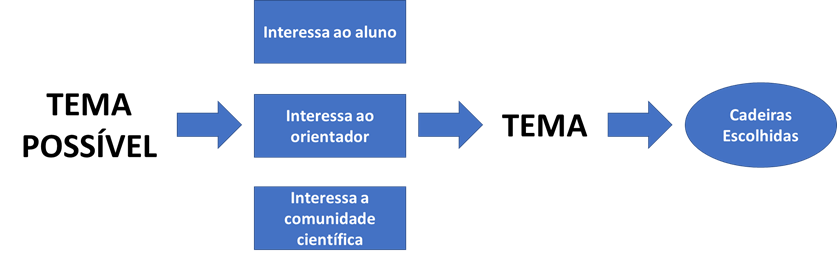
\includegraphics[width=0.9\linewidth]{Images/escolhatemacadeiras}
    \caption{Escolhendo tema e cadeiras. Fonte: o autor}
    \label{fig:escolhatemacadeiras}
\end{figure}


\section{O que é uma Contribuição Original}

Um dos requisitos da tese de doutorado é possuir uma contribuição original.

Eu confesso que contribuição original não é uma definição muito clara. Vamos analisar, então, o que é uma contribuição.

A professora Marta Mattoso diz que :
\begin{itemize}
\item	“Uma contribuição é um resultado que pode ser útil para outras pessoas.”
\item	“O resultado é uma novidade e não poderia ser afirmado sem o desenvolvimento da tese.”
\end{itemize}

Ou seja, uma contribuição pode se algo como encontrado na lista a seguir, levemente ordenada da maior para a menor e de forma não exaustiva.
\begin{enumerate}
\item	A solução de um problema em aberto;
\item	Uma melhoria comprovada a alguma prática da área;
\item	A proposta de uma metodologia, método ou processo que resolva um problema do mundo real, com uma abordagem científica;
\item	Aplicar uma prática da área em uma área de aplicação, de maneira não trivial;
\item	A investigação de um problema que descobre novas evidências na área;
\item	A criação de sistemas complexos envolvendo várias práticas até antes isoladas, com um resultado científico palpável;
\item	A comparação e análise de diferentes soluções computacionais para o mesmo problema, com consequente desenvolvimento de solução que as agregam de alguma forma;
\item	O levantamento de uma história, ou o estudo de casos, que trazem contribuição original para o entendimento de como algo aconteceu ou acontece, sempre de acordo com metodologias reconhecidas;
\item	A criação de novas bases de dados que podem servir para outros trabalhos.
\end{enumerate}

Porém, ao contrário de outras áreas, no Programa de Engenharia de Sistemas e Computação, e em toda COPPE, não é considerada uma contribuição;
\begin{itemize}
    \item 	Fazer a compilação de dados ou informações já existentes (como a criação de um review da área);
    \item	Desenvolver aplicações convencionais com software disponível amplamente;
    \item 	Desenvolver protótipos com tecnologia amplamente conhecida e divulgada.

\end{itemize}

Veja que a tese tem que comprovar a contribuição. Não basta dizer que algo é bom e original, é importante poder provar que é melhor (mesmo que dentro de alguns casos) e que não há outro resultado igual, ou ainda que abre um caminho novo de pesquisa.

\section{Como encontrar uma Contribuição}

Normalmente em uma tese de computação existe um problema, uma solução e uma comprovação ou validação da solução.

Assim, uma tese pode apresentar contribuições nessas três áreas. Lidando com o problema, podemos encontrar novos problemas ainda não tratados e modelar de formas diferentes problemas já tratados.

Na solução, podemos aplicar técnicas já existentes em problemas ainda não tratados com elas ou inventar novas técnicas. Finalmente, podemos trabalhar arduamente nas técnicas de comprovação de nossos resultados, principalmente quando esses resultados são experimentais ou empíricos\footnote{Em soluções teóricas é necessário provar que a solução é verdadeira, porém isso normalmente é parte da própria solução. Porém, existem teses teóricas que apresentam novas formas, mais simples, de provar um teorema já provado}.

O importante é ter um problema bem claro. Esse problema pode já ter sido proposto antes, ou pode ser levantado. Uma maneira de levantar problemas é estudar soluções já existentes e ver quando elas falham, ou que lacunas elas têm.

Listar as falhas ou lacunas de uma situação atual é um bom método de descobrir onde você pode trabalhar. As lacunas podem ser elencadas, algumas podem ser selecionadas, e toda a tese construída em torno desse conceito.

Muitos alunos querem começar pela solução, algo do tipo “quero usar a técnica X”. Esse não é um bom caminho, apesar de já ter funcionado para algumas pessoas. Porém, o que acontece normalmente é que o aluno fica com uma solução a procura de um problema e não tem como comprovar a qualidade ou a utilidade de sua solução.


\section{Pensando sua Tese}

Várias técnicas podem ser usadas para você pensar sua tese.

Algumas técnicas são muito úteis. Uma delas é a \gxdefine{5W2H}, responder as perguntas: Why, What, Who, When, Where, How e How Much. Essa é das técnicas mais gerais e mais úteis. Principalmente se perguntar “Por que estou fazendo isso” e “Quem vai ser beneficiado” permitem justificar plenamente o trabalho de sua tese, fazendo com que ela não fique perdida em um contexto vago.  A Figura \ref{fig:5w2h} mostra algumas perguntas possíveis nessa técnica.

% TODO: \usepackage{graphicx} required
\begin{figure}[hbt]
    \centering
    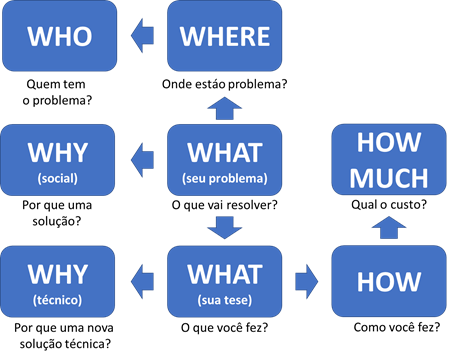
\includegraphics[width=0.7\linewidth]{Images/5w2h}
    \caption{Perguntas que devem ser respondidas antes de iniciar uma tese. Fonte: do autor.}
    \label{fig:5w2h}
\end{figure}




Algumas teses atuais têm proposto lacunas no estado da arte, e a partir dessas lacunas geram questões de pesquisa, que por sua vez podem gerar objetivos gerais e específicos. Esse é outro bom quadro teórico para trabalhar.

Entre meus alunos, o uso da \gxdefine{Design Science Research} (\gxdefine{DSR})\citep{Pimentel2020} também fornece caminhos para pensar sua tese . Eu estou me tornando cada vez mais um adepto dessa metodologia, dessa forma de fazer Ciência, que é realizada por meio de vários processos mais detalhados. Ou seja, não existe um método científico DSR, ele é mais uma filosofia de trabalho que fornece parâmetros para estabelecer um método específico.



Outra técnica possível, é desenhar um \gxdefine{Project Model Canvas}\footnote{\url{http://www.projectmodelcanvas.com/}} . Essa é uma proposta de José Finocchio Júnior e tem uma representação visual interessante, apresentada na Figura \ref{fig:pmc}.

% TODO: \usepackage{graphicx} required
\begin{figure}
    \centering
    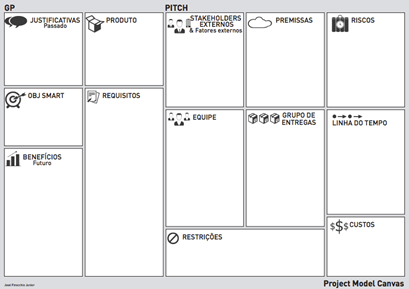
\includegraphics[width=0.7\linewidth]{Images/PMC}
    \caption{Representação do Project Model Canvas de José Finocchio Júnior (CC:BYNOND)}
    \label{fig:pmc}
\end{figure}


   \section{Como descrever o que é a tese}

Algumas coisas são importantes para você definir sua tese.

Primeiro, você tem que \textbf{conhecer um problema} e o \textbf{estado da arte da solução} do problema. Se seu orientador trabalha com o problema, você ainda tem que conhecer bem o trabalho que ele tem feito, para entrar realmente no grupo.

Segundo, é interessante que você consiga dar um \textbf{valor} a esse problema\footnote{Você pode ouvir uma aula sobre valor em \url{https://youtu.be/aOQQHGzC-YE}, ou ler o capítulo sobre valor escrito em \url{https://github.com/xexeo/MaterialEducacional}} . O valor pode ser econômico, como a diminuição de um custo, pode ser um valor acadêmico, como um teorema em aberto a muito tempo, ou pode ser outra forma de valor, como social ou histórico. Uma visão rápida de Valor, típica da Engenharia de Software, é procurar 3 coisas: aumentar o faturamento (benefícios), reduzir custos e melhorar serviços.

Terceiro, você deve ter uma \textbf{proposta de abordagem ao problema}. Isto significa que você deve entender caminhos possíveis para resolvê-lo e ter uma ideia das técnicas que pretende adotar.

Todas essas coisas podem ser descritas de várias formas, tanto ao longo do trabalho em apresentações como no texto final. Algumas abordagens mais tradicionais que outras.

\section{A descrição da tese na introdução}

Na introdução da sua tese deve existir uma descrição do que ela é e que deixe o leitor totalmente ciente do que vai encontrar durante a leitura.

Por exemplo, é importante \textbf{definir o problema} que a tese trata. Esse problema deve ocorrer dentro de um \textbf{contexto}. Também deve ficar claro o \textbf{objetivo} da tese. Esse objetivo pode ser dividido em \textbf{questões de pesquisa}, que devem levar gradativamente ao objetivo, ou pode gerar \textbf{conjecturas} que precisam ser comprovadas ou pelo menos validadas, já que certas conjecturas são difíceis de serem comprovadas de forma absoluta, devido a incluírem, por exemplo, aspectos do comportamento humano.

Costumamos, reservar o termo \textbf{hipótese para conjecturas que podem ser provadas com experimentos} que incluem uma hipótese nula, por meios estatísticos, ou provada, ou negada, por meio de um teorema. Chamar de hipótese, no corpo da tese, algo que não pode ser comprovado dessa forma, cria uma expectativa errada no leitor. Caso não haja uma comprovação formal, devemos evitar o termo hipótese e usar outros como conjecturas ou questões de pesquisa.

Podem ser necessárias também a elaboração de uma ou mais \textbf{premissas}, que são afirmações consideradas válidas a priori para sua tese. Premissas não são questionadas ao logo da tese, e sim assumidas como válidas. Claro que se espera que as premissas tenham alguma evidência, ou seja, não sejam facilmente falseáveis.

\chapter{O Seu Objetivo}

Vamos deixar bem claro:

\gxatencao{o seu objetivo é defender a tese.}


Uma tese \textbf{não} é um trabalho completo que vai dar a melhor solução do mundo para o problema mais importante que existe.

Na Coppe, uma tese tem objetivos definidos da seguinte forma :
\begin{itemize}
\item	``A Dissertação de Mestrado deverá demonstrar a aptidão do candidato para desenvolver atividades de pesquisa no tema escolhido e configurar uma contribuição significativa para o conhecimento na área correspondente''
\item	``A Tese de Doutorado deverá apresentar características de originalidade, demonstrando a aptidão do candidato para desenvolver atividades de pesquisa, e configurar uma contribuição significativa para o conhecimento nas áreas escolhidas de pesquisa''
\end{itemize}

Ou seja, sua tese tem que ser uma \textbf{contribuição} para a área e, no caso do Doutorado, apresentar características de originalidade. É comum, no PESC, que uma tese de mestrado já apresente essas características, mas não é necessário.


Além disso, sua tese deve \textbf{acabar dentro do prazo}.

Alguns ditados que recolhi entre amigos orientadores e orientados deixam bem clara a importância de terminar a tese:


``Tese não se termina, se entrega.''

``Tese boa é tese que acaba.''

``Você quer salvar o mundo ou tirar o título?''

Essas, e outras variações, são necessárias porque é comum o autor da tese achar que precisa “resolver o problema do mundo” ou que deve fazer uma tese perfeita. Isso é impossível, pois a tese está limitada em tempo.

Uma característica importante sobre teses de Doutorado: ao contrário do que muitos alunos pensam, uma tese que deixe muitos caminhos abertos é muito boa. Se isso acontece, o novo doutor é capaz de construir sua carreira, pelo menos inicialmente, resolvendo os problemas que ele mesmo descobriu ou tornou solucionáveis.

A professora Ana Regina Cavalcanti da Rocha costuma dizer:

\gxatencao{A Tese de Doutorado não é o último trabalho da vida de aluno, mas sim o primeiro trabalho da vida de pesquisador.}



\chapter{Conhecendo Suas Necessidades}

Antes de começar um projeto de mestrado ou doutorado, o aluno deve estar ciente de suas necessidades, limitações, restrições, capacidades e habilidades. Tudo isso deve ser levado em conta na sua preparação e mesmo na escolha se é o momento certo para realizar essa empreitada.

Em especial, quero chamar atenção às necessidades. Um trabalho de extrema repercussão é o estudo de Maslow  sobre a hierarquia de necessidades das pessoas\footnote{Esse trabalho também foi muito criticado, mas certamente podemos utilizá-lo para exemplificar o fato de que você tem que estar bem em vários sentidos para ter a calma necessária para fazer sua tese.}. Ele é facilmente compreendido a partir da “pirâmide de Maslow”, que apresento na Figura \ref{fig:maslow}.

\begin{figure}
	\centering
	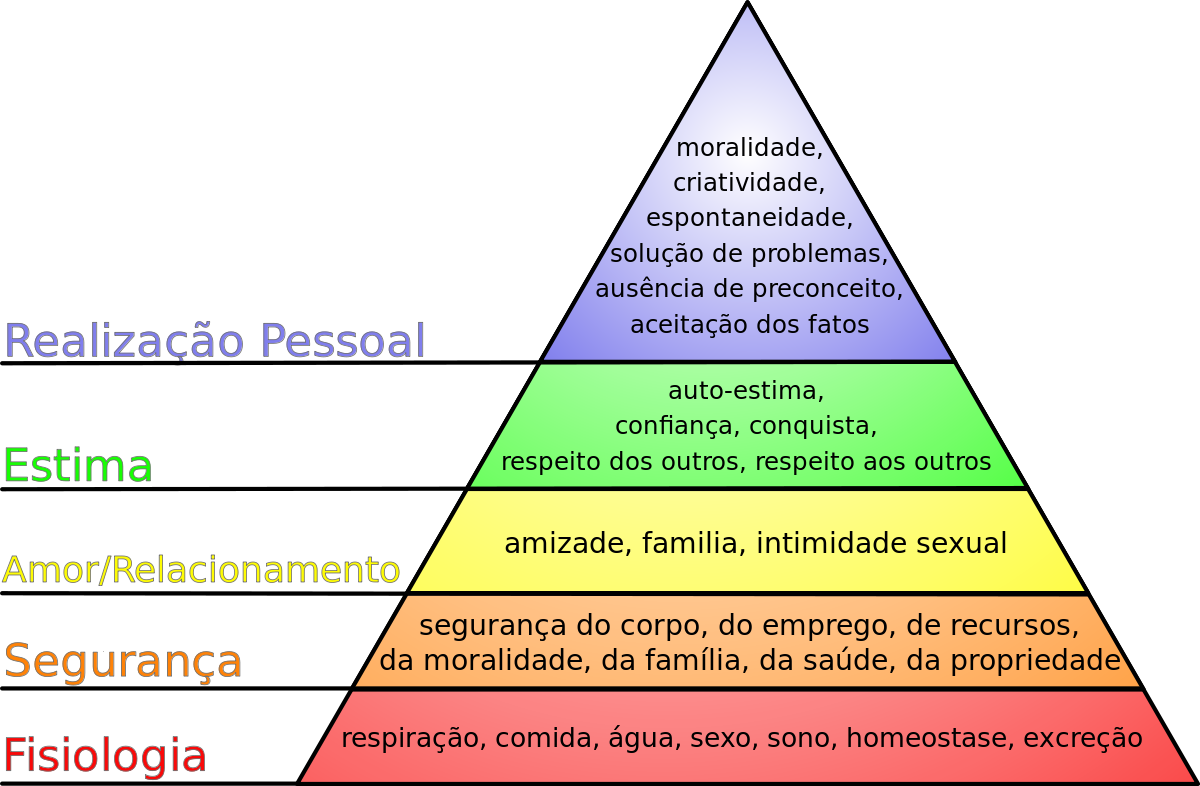
\includegraphics[width=0.7\linewidth]{Images/1200px-Hierarquia_das_necessidades_de_Maslow.svg}
	\caption{A pirâmide de Maslow.}
	\label{fig:maslow}
\end{figure}


Como se pode ver na Figura \ref{fig:maslow}, as necessidades são divididas em grupos e um grupo serve de base para todos os grupos superiores. Assim, as necessidades de realização pessoal (como fazer uma tese) são dependentes de todas as outras. 

Desse modo, podemos concluir que, para fazer uma pós-graduação, você deve garantir antes que tenha uma “boa base na pirâmide”. Isso significa garantir sua saúde, o modo de se manter, seus relacionamentos e sua autoestima.

Mesmo que você tenha começado sua dissertação ou tese em uma situação ideal, o longo prazo desse projeto, de 2 a 5 anos, implica em mudanças tanto no ambiente a sua volta quanto na sua própria vida. Alunos se casam, tem filhos, ficam doentes, se curam, precisam de mais dinheiro, se separam, trocam de emprego, tudo pode mudar nesse espaço de tempo.
Podemos citar como exemplo de acontecimento totalmente inesperado, e que afetou a todos em 2020/2021, a epidemia da Covid-19. Quantas vidas não foram mudadas? O impacto na vida dos mestrandos e graduandos foi muito variado e colocou um grande desafio para orientandos, orientadores e as instituições.

Voltando a pirâmide, ela indica que qualquer problema em uma camada inferior afeta diretamente a camada superior. Você deve estar consciente dessa estrutura e saber que problemas de qualquer tipo sempre afetarão seu rendimento na camada do topo, seja ocupando seu tempo, seja ocupando sua mente. Cabe ao aluno perceber e controlar o grau desse efeito, e quando necessário interagir com o orientador.

Por isso não hesite em procurar seu orientador e avisá-lo do que está acontecendo com você. Mesmo que ele não possa ajudá-lo no problema específico, ele compreenderá e tentará ajudar no que for possível. 
Exemplos típicos de coisas que acontecem na vida de um aluno: um novo emprego ou uma situação de desemprego, troca de chefes que afeta a liberação ou o interesse da empresa, doenças mais ou menos graves consigo ou com parentes, perda de acesso aos dados prometidos por alguém, gravidez, casamento, etc.

O orientador não é um sargento empurrando você em uma marcha forçada. Ao contrário, ele é o guia que evita que você se perca em uma exploração. Ele está ali para auxiliá-lo nos percalços do caminho, até mesmo para dizer que está na hora de parar e tentar em outra expedição. 
Uma relação aberta com o orientador é uma das mensagens que quero passar nesse texto. Ela vai facilitar sua vida e chegar ao seu objetivo.

\chapter{As Partes Interessadas na Sua Tese}

Toda tese é um projeto. As boas práticas de projeto sugerem que você levante, no início no projeto, e controle e gerencie, ao longo do projeto, as partes interessadas no projeto.
Mas o que são as partes interessadas? Não seria apenas você, ou você e seu orientador, as únicas partes interessadas?

Uma parte interessada é qualquer pessoa ou grupo que afete ou seja afetado pela sua tese, de verdade ou por percepção. A partir dessa definição vemos que existem muito mais partes interessadas.

Por exemplo, todos que se relacionam de maneira afetiva no dia a dia com você serão afetados pela sua tese, e alguns afetarão. 
Sua disponibilidade de tempo e atenção passará a ser dividida com a tese. 
Vários momentos que antes eram livres passarão a ser ocupados com pesquisas, leituras, programação, experimentos e outras atividades. 
Isso pode afetar os seus relacionamentos e você deve prestar atenção para que não prejudique fortemente sua vida pessoal.

Gostaria de contar o caso de um doutorando que mantinha um escritório fechado, para evitar que fosse desorganizado. 
Seu filho pequeno, ao ver a porta aberta, entrou e fez a maior confusão, porque tinha “raiva” do pai ficar no escritório e não com ele.

O \textbf{principal interessado normalmente é você}. Mas não apenas o você científico ou profissional, mas o você “completo”. Não só você afeta a tese, pois o sucesso dela depende do seu esforço, mas será também afetado por ela. O stress da pesquisa, da defesa, da dívida constante de trabalho, já causou problemas de saúde, física e mental, para muitos. Estudos mostram alarmantes  graus de depressão entre alunos de pós graduação~\citep{walker2015}.

O \textbf{orientador é outra parte interessada óbvia}. Todo orientador realmente quer que todos orientados defendam sua tese. Porém são também guardiões da qualidade do diploma, logo querem que a tese seja boa. Um bom orientador deve reprovar um aluno que não alcance os padrões acadêmicos de sua instituição, mas isso sempre é feito com desgosto. Mais de uma vez compartilhei com colegas a sensação de tristeza de ter um aluno que prometia resultados, mas não consegue, por um motivo ou outro, atingir um padrão de qualidade que garanta sua defesa.

Os membros da banca darão a palavra final da aprovação da sua tese. A tese deve atender padrões de qualidade, de honestidade científica, e eles são a barreira final. Muitas vezes seu orientador sinalizará: você precisa atender os padrões da banca, tem que ser capaz de convencer o leitor.

Depois desses grupos básicos, temos outras partes interessadas. Seu programa, os órgãos de fomento, a universidade, a sua comunidade científica e a sociedade em geral. Todos eles devem ser atendidos. 

Cabe então, a você, ao iniciar sua tese, pensar em como vai atender a todos. Seu orientador pode ajudar.

\section{Sua Família}
Família e tese são quase tão incompatíveis como trabalho e tese. A tese exige atenção. Nem sempre esposa, marido, filhos e filhas estão preparados para perder parte do tempo da atenção que lhe é normalmente dispensada para uma atividade intrinsecamente solitária.

Ninguém pode ajudar o candidato em sua tese. 

A primeira coisa a lembrar é que você precisa também dar atenção à família. Se decidir estudar todo domingo, por exemplo, saia com as crianças de manhã cedo e só depois comece a estudar. 

Aproveite os momentos de descanso para fazê-lo com sua família. 

Antes de começar uma tese, converse com sua família. Explique a necessidade de tempo, apoio e compreensão. Se necessário, deixe acordado desde o início que tempo será “integral” da família e não pode ser tocado. 

A hora de dormir com as crianças, o dever de casa, o cinema no sábado, o jantar romântico, tudo pode ter seu lugar se houver alguma organização de sua parte. 

\section{Seu Trabalho}

Se você trabalha, está em desvantagem. Em primeiro lugar, a pós-graduação não foi pensada, originalmente, para quem trabalha, mas sim para quem se dedica exclusivamente a pesquisa. 

Além disso, mesmo que seu empregador ou seu chefe tenha prometido a liberação, deixá-lo realizar seu sonho, ele realmente precisa que você trabalhe e ganhe dinheiro para a empresa. Isso significa que todas as promessas do seu empregador serão esquecidas com o tempo.

Algumas empresas liberam você para fazer sua tese. Para sermos justos, uma liberação de 4 anos, 2 para o mestrado, atende às necessidades de qualquer aluno (mesmo que você tenha mais prazo). É vital acabar a tese antes do final da liberação. Voltar para o trabalho sem terminar a tese não só atrapalha o fim dela como pode ser considerado por seus colegas como uma espécie de “derrota”, atrapalhando sua carreira. A pior situação possível seria você voltar e nunca acabar a tese! 

Também é comum que o aluno seja liberado para as cadeiras, mas não para o desenvolvimento da tese. Isso é um mau sinal. Caso seja liberado para as cadeiras apenas, tente pelo menos que o tempo de estudo seja incluído nessa liberação. Normalmente aconselhamos o aluno a considerar que o tempo de estudo para uma cadeira é, no mínimo, duas vezes maior que o tempo de aula. Isso significa que para cada hora de aula você teria que ter mais duas horas liberadas, totalizando três horas! Você pode colocar algumas dessas horas de estudo a noite ou no fim de semana, mas não todas.

É importante que você tenha por escrito todas as promessas da companhia, assinadas por uma pessoa com autoridade sobre seu chefe imediato, pelo Diretor de Recursos Humanos ou pessoa comparável.
Se você pertence a uma instituição com atenção curta, que toda hora muda de foco, seus problemas serão maiores. Quanto menor a sua empresa, maiores serão seus problemas. Se seu cargo envolve viagens constantes, seus problemas serão tão grandes que talvez seja impossível você realizar seus cursos ou defender a sua tese.

Se você trabalha na Universidade, então certamente terá mais chances e muito menos problemas. Se você pretende arranjar bicos durante o curso, procure trabalhos ligados à educação.Lembre que, a princípio, investimento na pós-graduação tem muito mais valor que o salário que você deixa de ganhar. 

\section{Os Órgãos de Fomento}

Se você ganha uma bolsa de algum órgão de fomento, como FAPERJ, CAPES e CNPq, você tem a responsabilidade legal de acabar a tese. 
Apesar de não ter sido a prática por muito tempo, atualmente há investigações e pedidos de restituição dos valores pagos como bolsa para alunos que não terminaram suas teses e não possuem uma justificativa.

Atenção também a taxa de bancada. Ela não é um adicional a tese, mas uma verba destinada a gastos na sua pesquisa e que devem ser comprovados. Você terá que prestar um relatório final e pode ser auditado.



\chapter{Que Tipo de Aluno Você É?}

A tese é um projeto de uma só pessoa. Seu orientador, por mais interesse que tenha no assunto, não vai fazê-la por você. Isso seria, inclusive, antiético e ilegal.


A responsabilidade é basicamente sua e o sucesso será prioritariamente seu. Logo, a pessoa mais importante nesse projeto é você, pois é a única que pode completá-lo. Compreender a si mesmo é um fator importante nesse processo. Entender suas características, sejam elas positivas ou negativas, ajudará a alcançar seu objetivo.


Uma maneira de compreender a si mesmo é conhecer estereótipos comuns das pessoas e ver até que ponto você se encaixa nesses estereótipos. 


Existem muitos tipos de alunos. Um orientador, com o tempo, desenvolve sua fórmula pessoal para tratar cada um deles. No texto a seguir, apresentarei alguns estereótipos. Raramente um aluno segue fielmente um desses estereótipos, mas eles servem como referência.


Apresentarei também algumas maneiras de se autoavaliar. Fique certo que muitos irão avaliar seu desempenho, principalmente seus orientadores. Muitas vezes receberá críticas, algumas justas, outras não. Entender a si mesmo e entendendo por que as pessoas o percebem de certa forma o ajudará a progredir.


Os alunos têm diferentes graus de dependência, ou independência, do orientador. A maioria dos alunos passa, durante a tese, por vários desses “graus”. Vamos analisar como funcionam os alunos estereotipados: o totalmente dependente e os totalmente independentes.


7.1	O estereótipo independente


O aluno totalmente independente é normalmente uma pessoa com interesses bem específicos. Escolhe um tema que o orientador pode auxiliar, mas não é necessariamente especialista. Sua relação de orientação é feita a partir da comunicação de tempos em tempos, ao orientador, do que está fazendo. Nessa conversa, tem sempre uma proposta de solução quando apresenta um problema e procura conhecer a opinião do orientador. 


Tive bons alunos desse tipo. Talvez todos eles tenham se envolvido, em alguma parte da tese, em problemas.


Um dos problemas que podem acontecer é que esse aluno, por se manter distante do orientador, tanto fisicamente quanto em relação ao tema de tese, não consiga imprimir um ritmo adequado sozinho. Isso se torna mais crítico quando o aluno tem alguma dificuldade pessoal grave e acaba “sem tempo” de informar o orientador.


\gxatencao{O aluno deve informar imediatamente ao orientador de qualquer problema pessoal que esteja dificultando ou impedindo seu progresso.
}

Principalmente com problemas emocionais, de saúde e financeiros graves, com si mesmo ou com sua família, o aluno deve informar o orientador e tomar com ele decisões como continuar trabalhando, ou suspender o trabalho ou até mesmo, e muito raramente, abandonar a tese. 

\gxatencao{O importante é que o aluno traga o problema ao orientador antes de criar um problema com seu prazo ou com suas avaliações}.


Outra coisa que pode acontecer é o aluno independente achar que o orientador o abandonou. Ele nunca fala com o orientador e, nas raras vezes que fala ou tenta falar, o orientador está muito ocupado. O orientador pode achar que o aluno o abandonou também, já que o aluno nunca o procura. Na verdade, pode ser que ambos tenham razão. 


Se houver alguma comunicação entre os dois e essa comunicação for clara, e a iniciativa do aluno for boa, a tese deve ser concluída. Se o aluno perder a iniciativa, o orientador terá trabalho para recolocá-lo nos trilhos, talvez não consiga. Se a comunicação for pequena o aluno corre o risco de querer fazer coisas demais e não acabar a tese ou fazer tudo errado, pois não sabe algum detalhe importante que o orientador já estudou.


No limite, alguns alunos desprezam a orientação, acham que o orientador não sabe o que está fazendo, ou simplesmente não ligam para a orientação.


Isso é péssimo. O orientador é mais experiente que o aluno e, se não tem a percepção localizada do assunto, por estar estudando menos o tema que o aluno naquele instante, tem a percepção generalizada bem mais apurada que a do aluno. Por isso que um é orientador e o outro aluno.


Um ditado típico da minha família é:


\gxatencao{O diabo não é perigoso por ser mais inteligente. 
O diabo não é perigoso por ser mais forte. 
O diabo é perigoso porque é mais velho.}


O orientador é mais velho, ou pelo menos está há mais tempo na área. Ou seja, o aluno independente tem muitas características boas, porém tem um risco muito alto.


\section{O estereótipo dependente}


Do outro lado do espectro, existe o aluno totalmente dependente. Esse aluno não faz nada sem perguntar ao orientador. Não tem ideias próprias. Desenvolve trabalhos a partir da orientação do orientador e fazendo implementações segundo algoritmos definidos pelo orientador. Nunca perde o contato. 


Supondo que esse aluno é competente, ele é um aluno de risco baixo. Tem grandes chances de acabar a tese, porque faz tudo que o orientador manda e o orientador deve saber em que direção vai à tese. 


Os riscos em relação a esse aluno ocorrem se orientador estiver em uma fase muito criativa, mas sem foco ou sem tempo. 


Outro risco importante é o aluno não se identificar com a tese, porque foi escolhida pelo orientador. 


\section{O aluno real}


Se você olhar as descrições acima com cuidado vai perceber algo estranho: o aluno independente, supostamente o melhor aluno, é o que corre mais riscos. Isso acontece porque tanto a construção de uma dissertação ou tese quanto a orientação são processos. Quanto mais o orientado faz parte do processo, mais chances têm que terminá-lo de forma satisfatória.


Obviamente, nenhum aluno é totalmente independente ou dependente. Pessoalmente, tive boas relações com alunos em vários pontos do espectro. O importante é que o aluno permaneça em contato com o orientador. 


Aviso aos orientados que é o aluno que se mantém em contato com o orientador, não o inverso. É o aluno que deve procurar, marcar reuniões, trazer o trabalho. É o orientado que deve esperar pelo orientador na porta de sua sala. O orientador possui vários alunos e tarefas, dificilmente consegue controlar a frequência de cada um. Lembre-se, você é um dos alunos de seu orientador, enquanto seu orientador é o único que você tem.


\gxatencao{O aluno deve se manter em contato com o orientador.}


Uma história pessoal: quando queria falar com meu orientador sozinho, sem interrupção, eu pegava uma carona. Era a única forma de ter um “tempo só para mim”. E nem sempre dava certo.


\section{Como se avaliar quanto à independência}


Tente responder as seguintes perguntas:
\begin{itemize}
	\item Eu converso com meu orientador com uma frequência fixa?
	\item Quantas vezes por mês eu converso com meu orientador?
	\item Meu orientador é capaz de dizer em que ponto eu estou na minha tese?
	\item Meu orientador é capaz de falar sobre minha tese?
\end{itemize}





\chapter{Hábitos e Práticas}


\section{Ler}


A leitura é a única forma do candidato a um título alcançar a maturidade necessária para defendê-lo. Muitos alunos têm uma boa ideia e acreditam que realizá-la e descrevê-la caracteriza uma tese. Isso não é verdade. 


\gxatencao{O aluno deve ler.}


Uma tese tem que ser colocada no contexto científico atual e comparada com os trabalhos já realizados sobre o assunto ou sobre temas similares ou análogos. Deve ficar claro, na tese, qual a colaboração que o trabalho traz a ciência. Obviamente, só é possível fazer isso se o aluno tem um conhecimento da área, que deve ser, na maior parte das vezes, até mesmo superior ao conhecimento do orientador.


Quando o aluno não lê o suficiente isso fica muito claro para o orientador. Há uma falta de capacidade de argumentação, uma falta de base teórica para o trabalho. Um dos principais sinais de maturidade que um orientador percebe é a capacidade de argumentação baseada em evidências científicas.


É importante notar que não basta ler, mas é necessário ler publicações atualizadas (além dos textos clássicos da área).


Se você achar que está lendo pouco, ou se seu orientador reclamar disso, aqui estão algumas dicas:

\begin{outline}	
\1	Levante uma lista de congressos e revistas relativas à área de sua tese.
\2	Faça um mix com o máximo possível de publicações da área específica com publicações importantes da área mais geral
\1	Obtenha os últimos cinco anos desses congressos e revistas.
\1	Liste todos os artigos disponíveis que possam servir para sua tese
\1	Obtenha esses artigos
\1	Leia os resumos e os organize de alguma forma, priorizando a leitura
\2	Procure tutoriais e reviews para o início da leitura
\2	Leia alguns artigos clássicos citados nos artigos obtidos
\2 Leia os artigos específicos, com foco nos mais atuais
\1	Mantenha o controle dessa lista e faça o acompanhamento com o orientador.
\end{outline}

A maioria dos textos de metodologia científica recomenda o fichamento dos artigos lidos. Essa prática é importante, porém não é mais necessário usar fichas. Você pode usar um banco de dados, um sistema de referência ou até mesmo um ou mais arquivos de documento, como arquivos Word. Até mesmo “Post-it” podem gerar um bom sistema de fichamento. 


\subsection{O Aluno que só lê português (e não conta ao orientador)}


Dificilmente você será aceito no mestrado se sua capacitação em inglês não permite uma leitura em ritmo razoável, porém isso pode acontecer.


Nesse caso, deixe bem claro ao orientador sua dificuldade. Esconder qualquer dificuldade de leitura ou compreensão, seja ela de inglês ou de alguma matéria específica, fará com que seu orientador avalie sua dificuldade como falta de dedicação.


O resultado é que, em vez de o orientador ajudá-lo nessa dificuldade, ele tornará as coisas cada vez mais difíceis.


Por sinal, se esse for seu caso, entre imediatamente em um curso de inglês. Qualquer melhoria, junto com a leitura de textos da área, implicará em um rendimento maior do seu trabalho. Existem cursos gratuitos ou muito baratos na universidade.


\section{Escrever}


É quase impossível seguir uma carreira acadêmica em qualquer área de sem escrever bem, pelo menos em português. 


Se você acha que escreve mal, ou se os outros acham que escreve mal, tente corrigir o mais rápido possível. Faça cursos e se esforce. Muitos alunos simplesmente acham “normal” um profissional de área técnica escrever mal. Isso demonstra uma falta de compreensão das necessidades do mundo real: apresentar e defender, de forma clara, suas ideias. 


Como diria o Chacrinha\footnote{É provável que alguns dos leitores mais novos não tenham conhecido o “Chacrinha”. Ele foi por muitos anos um apresentador de programa de auditório de muito sucesso, usando uma fantasia e utilizando bordões engraçados. Certamente foi uma das figuras mais conhecidas na TV brasileira do século XX.}: 


\gxatencao{Quem não se comunica, se trumbica}


Uma das principais indicações da educação de uma pessoa é sua capacidade de se expressar em sua língua mãe.


Ao estudante universitário, essa característica é muito desejada. Ao aluno de mestrado e doutorado, é indispensável.


Contribuição de um aluno que aprendeu a escrever.

\quote{Só consegue escrever quem consegue dizer o que pensa e quer.  Fale, diga o que pensa, conte para seu orientador suas ideias e busque clareza ao dizer.

Escreva simples.  Uma tese é, antes de qualquer coisa, uma coleção de folhas de papel com um monte de letrinhas em cima.  

Ler é, depois de falar, uma das melhores ajudas para quem quer aprender a escrever.  Ler tudo, de jornal a bula de remédio, passando por contos, poesias, história em quadrinhos, artigos e, naturalmente, uma tese ou outra de vez em quando.

Depois fica-se assim, querendo escrever em qualquer lugar, em qualquer oportunidade, em qualquer Wiki que se abra.

Desejo boa sorte a nós todos.

\textit{Bebeto}}



\chapter{O Orientador}


A função do orientador é orientar, mostrar caminhos, estimulá-lo a pesquisa, gerar problemas que você possa resolver. Ele também deve ajudar com a burocracia e com problemas relacionados à universidade. 


Não é função do orientador resolver os problemas da sua tese. Porém, ele pode, eventualmente, dar contribuições essenciais.


Alguns orientadores vão ajudá-lo a resolver problemas pessoais, provavelmente apenas com conselhos, mas não é essa sua função. Ele deve conhecer os problemas para entender a sua produtividade, mas não é sua obrigação resolvê-los. Se o faz, faz por vontade própria e solidariedade.


A relação orientado/orientador é muito variada, porém deve ser sempre cordial. Faça todos os esforços possíveis para não iniciar uma discussão pessoal com seu orientador. 


\gxatencao{O respeito é essencial}


A primeira coisa a entender é que o orientador não é orientador por ser mais inteligente que você, mas por ter mais experiência que você em uma área específica. Muitas vezes os orientadores são mais novos que os orientados e mesmo assim alcançam bons resultados. É claro que é importante que você respeite a inteligência do seu orientador, mas esse não é o fator de diferença entre orientado e orientador.


\section{Dificuldades comuns com os orientadores}


Certamente seu orientador o tratará com respeito, porém os seguintes problemas podem aparecer:

\begin{outline}
\1	O orientador não tem tempo para você


\1	O orientador não leu o que você escreveu


\1	O orientador não entende o que você faz
\end{outline}

\subsection{O Orientador sem tempo}


É comum um orientador ter pouco tempo disponível. Ele tem que dar aulas, participar de reuniões, orientar outros alunos e realizar atividades como pesquisa e consultoria. Você deve se adaptar ao tempo disponível de seu orientador. 


Algumas desculpas são inaceitáveis pelo orientador e entre elas está que “você não pode sair de seu trabalho nessa hora”. Afinal, você está ou não fazendo uma tese? É possível, porém, que seu orientador concorde em o orientar na casa dele, após o expediente, e, em casos excepcionais, no fim de semana. Não é o meu caso e acredito que, tirando condições excepcionais, não devia ser o caso de nenhum orientador.


Caso seu orientador tenha problemas graves na agenda, tente marcar um almoço com ele. Outra opção é conseguir um coorientador, outro professor da mesma área ou um aluno de doutorado, caso você seja aluno de mestrado. Muitos orientadores gostam de trabalhar no regime de dupla orientação.


\subsection{	O orientador que não leu o que você escreveu}


Se o orientador não leu o que você escreveu é porque não teve tempo ou esqueceu. Se ao encontrar seu orientador ele não tiver lido o que você escreveu, faça um resumo mostrando o texto para ele. 


\gxatencao{Sempre leve uma cópia do trabalho que você está fazendo para as reuniões. }


Aparecer em uma reunião sem isso é demonstrar desinteresse pela reunião, falta de preparação ou, pior, que você não fez nada.


Muitos orientadores leem um texto por alto e ficam com uma ideia muito clara do que foi feito. Principalmente nos casos de revisão bibliográfica e resultados demonstrados em gráficos, o orientador pode em 10 ou 15 minutos ter uma ideia clara do seu trabalho e contribuir para o seu desenvolvimento. 


É importante entender que o esforço do orientador é muito relacionado ao esforço do aluno. Alguns alunos parecem frustrados porque o orientador, na segundo ou terceira vez que eles aparecem com o trabalho no mesmo estágio, não estão dispostos a conversar por muito tempo ou dar ideias. Essa reação não é nada surpreendente, se você não faz o seu trabalho, o orientador não tem como fazer o dele.


\gxatencao{Um processo de orientação se baseia na evolução do trabalho do orientado.}


\subsection{O orientador que não entende o que você faz}


Das três situações que citei, essa é a mais difícil de resolver.


Não é raro que um aluno desenvolva um assunto de tese que foge dos conhecimentos do orientador. Nesse caso muitos orientadores coíbem o desenvolvimento da tese, enquanto outros buscam soluções de compromisso. Outros podem entender como uma oportunidade de abordar novas áreas. Na verdade, dependendo do assunto, a disposição do orientador pode mudar.


Uma coorientação pode, novamente, ser uma boa solução. Uma revisão bibliográfica também pode dar ao orientador as ferramentas necessárias para auxiliar no seu trabalho. Em geral, um orientador fica feliz se seu aluno sabe mais que ele sobre um assunto.


\section{Mais sobre os orientadores}


Os orientadores também passam por ciclos de alta imaginação e excessiva realidade. Muitas conversas serão “viagens” e outras serão “convocações para pôr o pé no chão”. De certa forma, essa é a tarefa do orientador. Se você estiver viajando pouco, ele vai tentar desenvolver os limites da sua imaginação, se você estiver passeando no espaço sideral, ele vai tentar trazê-lo de volta para a realidade.


As conversas com o orientador devem ser plenamente documentadas, pelo aluno, mesmo que o orientador faça isso. Se os dois estiverem documentando a conversação, compare as notas no final. 


\gxatencao{O aluno deve sair de cada conversa com uma lista de itens a fazer}


Se seu orientador não criar essa lista, pergunte diretamente quais devem ser seus próximos passos ou sugira você mesmo uma lista de ações. 


Entre duas sessões de orientação, seu orientador certamente mudará de ideia. 


\gxatencao{Nunca jogue fora um trabalho anteriormente descartado}


Caso um assunto previamente descartado como “ruim” seja considerado “bom” em uma reunião posterior, verifique em suas anotações o motivo da decisão anterior e discuta-os com o orientador. Porém, tente não questionar a mudança de opinião, pois isso só vai levar a um sermão sobre a necessidade de se ter uma mente aberta e pronta para mudanças. Revise os defeitos e qualidades da opção sendo estudada e tome uma nova decisão.


Existem muitos tipos de orientadores: o viajante, o amigão, o carrasco, o executivo, o objetivo etc. Todos esses têm suas vantagens e desvantagens, cabe a você descobrir quais os defeitos do seu orientador e evitar que eles tenham má influência na sua tese. Se seu orientador tem muitas ideias, você deve ser objetivo, se seu orientador é relapso com prazos, você deve cumprir todos. Orientadores são seres humanos e têm defeitos, muitas vezes graves. 


Só você pode evitar que esses defeitos influenciem na sua tese. Quanto aos seus defeitos, fique certo de que o orientador irá apontá-los no decorrer do relacionamento, algumas vezes até de maneira um tanto rude.


\section{Confiança no orientador}


O maior desejo do orientador é que o aluno termine a tese. É quase inconcebível imaginar que um orientador não deseje que o aluno complete o mais rápido possível e da melhor forma, o seu trabalho. 


Por que falo isso com tanta certeza? Porque os professores são avaliados, parcialmente, pela capacidade de fazer seus alunos defenderem suas teses e publicarem artigos sobre elas.


Alguns alunos, porém, imaginam que o professor está contra eles. Acham que estão pedindo trabalhos impossíveis, apenas para o benefício próprio, ou pior, para atrapalhá-los.


A verdade é que cada orientador determina um nível de qualidade aceitável para o trabalho do aluno. Esse nível é compatível com as características do aluno. 
Assim, um aluno capaz de fazer ótimos programas de computador, mas péssimo em teoria, é estimulado, e cobrado, a explorar suas qualidades ao máximo e a lutar, na medida do possível e do aceitável, contra suas dificuldades.


O orientador trabalha \textbf{sempre a favor do aluno}, dentro de algumas restrições pessoais e institucionais. 
Essas restrições envolvem a área de pesquisa, a qualidade do resultado, a dedicação ao trabalho e muitos outros fatores. 
Poucas vezes um orientador reprova ou abandona um aluno.
 Ele sempre tenta ao máximo encontrar um caminho de sucesso. 
 Essa é a tarefa principal do orientador.


Uma restrição importante que todo aluno deve estar atento é que a carreira acadêmica do orientador é fortemente, se não unicamente, influenciada pela quantidade e qualidade de suas publicações. 
O orientador é um professor que tem que arcar com muitas responsabilidades: aulas, administração da faculdade, orientação e escrever artigos. 
Assim, os orientadores normalmente esperam que o orientado os auxiliem na tarefa de escrever artigos. 


Os alunos que desejam seguir carreira acadêmica devem ficar especialmente preocupados em publicar, afinal, eles também serão julgados por sua capacidade de produção de artigos.


\gxatencao{Assim, o aluno deve estabelecer uma relação de confiança e colaboração com seu orientador.}


\section{A Escolha}


A escolha do orientador é um processo bastante complicado. Alguns alunos não têm essa opção, pois são selecionados desde o início para serem orientados por um professor. 


Você pode analisar um orientador de acordo com as seguintes facetas:

\begin{enumerate}
	\item 	Compatibilidade pessoal


	\item 	Assuntos comuns


	\item 	Qualidade como orientador


	\item 	Qualidade como professor


	\item 	Qualidade como pesquisador


	\item 	Opinião pessoal

\end{enumerate}

Existem muitas maneiras de iniciar essa seleção. Normalmente você deve ter como opção os professores com qual já fez alguma cadeira ou trabalho. Seus colegas mais antigos também são capazes de dar informações sobre os professores disponíveis. Além disso, muitas vezes outros professores podem recomendar um colega, de acordo com seus objetivos como aluno.


Um conselho importante é não se assustar muito com orientadores com fama de durões. Um orientador durão pode ser um ótimo orientador e manter você nos “trilhos certos”. Cuidado, porém, com os que tem fama de mal-educados.


\section{Problemas com o orientador}


Aconteceu! Você discutiu com seu orientador de forma irreconciliável ou se acha prejudicado fortemente. O que fazer?


Primeiro, respire. É importante parar para pensar, pois existe um registro histórico que é desfavorável a você: seu orientador já orientou diversos alunos e trabalhos, você não fez nenhuma tese.


É fato que todo relacionamento de longo prazo está sujeito a turbulências. Namoros e casamentos acabam, por que uma orientação não pode acabar? O problema é que, nesse caso, normalmente apenas um lado é prejudicado: o aluno.


Para resolver o problema temos que pensar em um escalonamento de soluções. 


Por incrível que pareça, a primeira pessoa que pode ajudá-lo é o próprio orientador. Tente marcar outra reunião e de forma educada dizer que não consegue mais trabalhar nas condições atuais. Lembre-se que, sendo a parte mais frágil, acusar pouco vai servir a você. Seu orientador então pode se propor a buscar um novo orientador ou um coorientador. Essa solução é a mais fácil.


A seguir, caso isso não funcione, você deve caminhar lentamente pelas instâncias superiores da instituição. Na COPPE existe um chefe de linha, a coordenação acadêmica e o coordenador, dentro do Programa. No nível de diretoria ainda existe o Coordenador Acadêmico e o Conselho de Pós-Graduação e Pesquisa(CPGP).




\chapter{Dedicação Para a Tese}


\gxatencao{A única maneira de se acabar uma tese é com dedicação.}


Dedicar-se significa reservar horas para seu trabalho de tese. A tese não pode ficar relegada às horas livres, pois essas tendem a sumir rapidamente. 


Dedicar-se significa se esforçar para obter informações, descobrir que informações são necessárias e manter um ritmo de trabalho constante no início e crescente do meio para o final. 


É importante estar preparado para dedicação exclusiva nos dias finais que antecedem a entrega da tese e lembrar de reservar alguns dias para fazer as correções solicitadas pela banca.


A melhor maneira de se dedicar é ter um plano de horários e obedecê-lo, planejar a tese como se fosse um dia de trabalho e cumprir o planejamento. Devo dizer que nunca vi alguém fazer isso, pois as necessidades do dia a dia acabam se encaixando com a flexibilidade dos horários de estudo e “bagunçando o coreto”. Mas aqui vão algumas dicas para organizar sua dedicação:

\begin{outline}
\1	Carga Horária


\2	Determine uma carga horária mínima por dia, por semana e por mês. Tente cumprir todas as cargas horárias. Nunca deixe a carga mínima do mês atrasar.


\1	Metas Específicas


\2	Defina metas específicas, principalmente quando relacionadas à parte do texto da tese e parte do software. Dê um prazo para essas metas. Tenha metas objetivas para cada final de período letivo.


\1	Horário de Trabalho


\2	Defina um horário de trabalho preferido. Você pode ser do tipo madrugador ou noturno. Aproveite a flexibilidade para trabalhar na hora que produz mais. 


\3	Ao longo do tempo, apesar de madrugador, passei a considerar que é mais produtivo que a tese seja seu primeiro trabalho do dia, de modo que você não esteja nem cansado, nem influenciado por outros problemas. Assim, recomendo a meus alunos que têm atividades paralelas acordar pelo menos uma hora mais cedo todo dia para trabalhar na tese.


\1	Aos que dormem tarde, garanto que com o tempo passarão a dormir mais cedo.
\end{outline}

\section{Avaliando Seu Trabalho}


Uma maneira de saber como seu trabalho está andando é avaliá-lo periodicamente. Todo dia se pergunte: eu fiz algo para atingir meu objetivo?


Duas perguntas são importantes em relação aos seus objetivos de tese:

\begin{outline}
\1	O que você escreveu?


\2	Tem relação ao seu trabalho escrevendo capítulos da tese, programas, especificações e artigos em revista. 


\2	Responda à pergunta: em quantos trabalhos desse tipo eu coloquei algum esforço hoje e produzi algum resultado palpável?


\1	Com quem você colaborou?


\2	Tem relação aos tipos de colaborações que você fez nesse dia, semana ou mês. Formas de colaboração possível são:


\3	Fiz algo para meu orientador?


\3	Fiz algo para um colega?


\3	Pedi algo para um colega? 


\3	Dividi algo com um colega?
\end{outline}

\section{Objetivos S.M.A.R.T.}


Um método interessante de criar objetivos em seu trabalho, ou em sua vida em geral, é lembrar do acrônimo S.M.A.R.T. Segundo essa teoria, um objetivo deve ser:

\begin{outline}
\1	S – eSpecífico (Specific)


\2	O objetivo deve ser específico e não generalizado. Ou seja, deve ser algo que pode ser claramente atingido. Um bom exemplo é “entrar em uma academia e me exercitar 3 vezes por semana” e não “malhar”. 


\1	M – Mensurável (Measurable)


\2	Deve ser possível avaliar que ele foi atingido. O exemplo típico é ótimo: “perder 5 quilos”.


\1	A – Atingível (Attainable)


\2	O objetivo tem que ser alcançável. Você tem que se propor a realizá-lo e tem que compreender suas dificuldades.


\1	R – Realista (Realistic)


\2	O objetivo tem que ser realista. Não adianta querer perder 50 quilos em uma semana. 


\1	T – limitado no Tempo (Time Bound)


\2	Você tem que dar um prazo para o objetivo acontecer. Por exemplo “Perder 5 quilos em 3 meses”.


\2	Alguns autores consideram T para “Tangível”, no sentido de ser algo que possa ser avaliado de acordo com os 5 sentidos (tato, paladar, visão, audição e olfato). 
\end{outline}

Relacionados à tese, bons objetivos podem ser:

\begin{itemize}
	\item	Escrever um capítulo de revisão bibliográfica de 15 páginas em um mês.
	
	
	\item	Escrever um artigo descrevendo a experiência realizada até dia 30 de setembro.
	
\end{itemize}


Devemos lembrar que os prazos que recebemos da instituição e de congressos e revistas são ótimos mecanismos para determinar nossos limites no tempo.



\section{Técnicas de Estudo e Trabalho}


Existem muitas maneiras de trabalhar e estudar, principalmente na frente do computador. Quero chamar atenção a uma técnica e uma teoria que são muito difundidas, mas que são opostas, respectivamente, Pomodoro, Flow (ou Fluxo).


Fluxo é uma teoria proposta por Mihaly Csikszenbtmihalyi que diz que existe um estado de alta concentração onde entramos em fluxo. O fluxo é um estado da mente onde estamos altamente focados no trabalho, não sentimos o tempo passar. Para alcançar o fluxo cada pessoa precisa de um certo tempo, que pode chegar a 30 minutos. Porém, se perdemos a concentração, saímos imediatamente do estado de fluxo e voltamos a precisar do mesmo tempo para entrar de novo nele. 


Seguindo esse caminho, é importante reservar momentos mais longos e com nenhuma interrupção. Se desligar do celular e das redes sociais é essencial para atingir o Fluxo.


Pomodoro é uma prática de estudo onde treinamos o cérebro para funcionar focado em curtos períodos. Tradicionalmente se usa 25 de trabalho por 5 de descanso por ciclo, mais 15 a 20 minutos de descanso depois de 3 ciclos. A principal parte dessa técnica é gerenciar as distrações.


Claramente a técnica Pomodoro interrompe o estado de fluxo. Não está claro qual escolher, talvez algumas tarefas sejam adequadas a procurar o fluxo e outras a técnica de Pomodoro. Pessoalmente eu reconheço minha capacidade de entrar em estado de fluxo quando faço tarefas como escrever algo ou programar, conseguindo grande concentração. Confesso que as vezes, ao sair do fluxo, tenho até dificuldade de entender de novo o código que escrevi. Já a técnica Pomodoro não funciona bem comigo, que tenho tendência a procurar desculpas para exceder o tempo de descanso, me envolvendo com outras atividades.


Sugiro aos leitores que se aprofundem mais nas duas técnicas, façam experimentos consigo mesmos e escolham a que mais se adapta ao seu estilo.


\section{Ambiente de Estudo}


Uma das coisas mais importantes é ter um ambiente de estudo onde você se sinta bem. Alguns preferem o silêncio, outros necessitam de música, cada um tem um gosto pessoal. Aqui vão algumas dicas: 

\begin{itemize}
\item	Tenha um computador próprio e exclusivo. 


\item	Lembre-se: você é um aluno de Computação, o mínimo que pode ter é um computador próprio.


\item	Isso também é uma defesa, já que você não quer que outros destruam sem intenção o seu trabalho.


\item	Tenha um ambiente de estudo em casa e um na faculdade. 


\item	Cultive esses ambientes, retirando dele tudo que pode atrapalhar sua concentração e usando-os prioritariamente. 


\item	Em cada início de período dê uma “arrumada” no seu computador, evitando assim problemas graves no meio do período. 


\item	Evite estudar em uma posição que leve ao sono. 


\item	Tenha uma estante reservada para o material de estudo. 


\item	Mantenha seus artigos organizados. Encaderne-os ou coloque-os em fichários, ou em diretórios organizados. Eu uso o software Calibre para todos meus PDFs, por exemplo.
\end{itemize}

\section{O Método do Tadeu}


Um dos alunos mais organizados que tive foi o Tadeu Classe. Ele me mandou esse relato sobre como se organiza.


\quote{Desde que comecei meu doutorado constantemente vinha percebendo que precisava organizar melhor as minhas tarefas. Sou um doutorando que não faz somente a sua pesquisa, pois preciso me manter na cidade onde vivo, e tenho outras atividades, como treinos esportivos, lecionar em instituições de ensino superior e trabalhar como analista de sistemas.}

\begin{figure}[hbt]
	\centering
	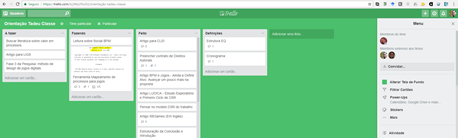
\includegraphics[width=0.7\linewidth]{Images/Trello}
	\caption{Imagem do Trello, software que o Tadeu usou durante sua tese. Fonte: imagem fornecida por Tadeu Classe}
	\label{fig:trello}
\end{figure}



\quote{Devido a isso, a minha desorganização vinha tomando conta, e não conseguia desempenhar nenhumas das atividades que realizava com qualidade. Um dos meus orientadores, a Profª. D.Sc. Renata Araujo da UNIRIO, sempre sugeriu desde o início dos meus estudos, que eu tentasse me organizar usando o programa Trello (https://trello.com/), que é um quadro virtual de atividades, onde você consegue organizar e grupos e ir colocando lembretes para a realização das atividades, porém, pessoalmente não gostei muito de usar a ferramenta. Pois mesmo organizando as tarefas, e o que eu precisava fazer, eu não lembrava de acessá-la e atualizá-la.}

\begin{figure}[hbt]
	\centering
	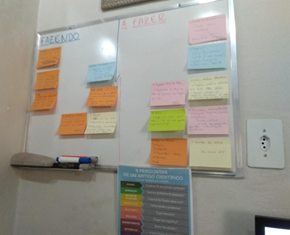
\includegraphics[width=0.7\linewidth]{Images/quadroorganizacao}
	\caption{Quadro de organização de Tadeu Class. Fonte: imagem fornecida por Tadeu Classe.}
	\label{fig:quadroorganizacao}
\end{figure}



Figura 4 - Trello: área de organização


Entretanto, me baseando no Trello e para que eu conseguisse organizar melhor os meus afazeres durando meu dia a dia como doutorando, analista de sistemas e professor, decidir colocar em meu escritório de trabalho um quadro branco. Neste quadro eu fiz a sua divisão em duas áreas (“A FAZER” e “FAZENDO”) no qual eu anexo “post-its” com as tarefas que eu preciso realizar [Figura 2], trocando entre os lados as prioridades, sendo que as tarefas que forem sendo realizadas, jogo o post-it no lixo. Meus post-its são coloridos, e cada cor indica o grau de urgência da atividade a ser realizada, por exemplo: laranja: URGÊNCIA, azul: PRECISAM SER FEITOS, rosa: FAZER ASSIM QUE SOBRAR UM TEMPO, amarelo: SEM URGÊNCIA, e verde: UM DIA EU FAÇO.




Figura 5 - Quadro de Organização


Desta maneira consegui ter um quadro de tarefas onde consigo organizar tudo o que precisa ser feito em meu dia a dia, com a vantagem de que o mesmo está sempre na minha frente fazendo com que eu sempre esteja olhando para ele. Minha produtividade melhorou muito desde então, e ele me auxiliou a entregar todas as demandas nos prazos corretos.



\include{Conteudo/OtimoBom}
\include{Conteudo/Publicando}
\include{Conteudo/MetodologiaCientifica}
\chapter{Ambiente Universitário}

É importante participar do ambiente universitário. Vá sempre a sua universidade, encontre seus colegas. Vá ao laboratório. Assista a seminários. Troque artigos.


Você não pode faltar de jeito nenhum aos seguintes eventos:
\begin{itemize}
    \item 	Eventos promovidos por seu orientador
    \item 	Eventos promovidos pelo grupo do seu orientador
    \item 	Defesas de tese orientadas por seu orientador
    \item 	Defesas de tese de seus colegas de turma
\end{itemize}

No final, quando você souber qual a formação de sua banca, procure defesas de tese com os mesmos integrantes. Isso ajudará você a conhecer a sua banca.

Seus colegas podem fornecer muita informação para você e você deve fornecer para eles também.

Não se torne um “capacitor” de informações, acumulando-as sem passar para ninguém. O pior tipo de pesquisador é aquele que sabe algo e não divulga.

\chapter{O Exame de Qualificação}

Praticamente em todos os programas de doutorado o aluno deve ser aprovado em um exame de qualificação para se tornar um candidato ao doutorado.

O exame de qualificação busca avaliar 3 quesitos:

\begin{enumerate}
\item	O aluno tem conhecimento suficiente para realizar o doutorado?
\item	O tema de tese conterá uma contribuição original?
\item	O tema de tese é factível?
\end{enumerate}

Um cuidado a ser tomado é não pensar que o exame de qualificação é como uma tese. Como documento, ele deve ser bem menor, como assunto, ele deve ser focado na proposição e na avaliação de viabilidade.

Como há um prazo máximo, os exames podem ser feitos em vários momentos da tese. Exames mais tardios exigem que o aluno já tenha trabalhado razoavelmente no tema. Há locais onde para o exame ser feito a tese já tem que estar toda estabelecida e só estejam faltando coisas como o experimento comprobatório.

Um exame feito mais cedo pode ser mais teórico, com menos contribuições já realizadas.
Para mim, um exame de qualificação deve ter pelo menos uma tentativa de solucionar o problema, ou uma investigação na dificuldade de fazê-lo, por meio de tentativas mais ou menos sofisticadas, dependendo do tempo que já foi gasto do prazo da tese.

\chapter{Resultados}

Só existe uma maneira verdadeiramente honesta de avaliar um trabalho científico: submetê-lo a revisão de seus pares. Por isso existe uma banca de mestrado e doutorado. Por isso cada vez mais é importante publicar seus resultados.

Na forma atual que alunos, professores e programas de pós-graduação são avaliados é impossível imaginar uma tese onde não houve uma publicação. A política correta de um orientador deve ser não permitir a defesa de uma tese que não tenha nenhum artigo publicado. Para isso dou dois motivos: se nenhum trabalho foi apresentado para a publicação, então o aluno não demonstrou interesse, se nenhum trabalho foi aceito, a tese não demonstrou capacidade.

Publicar é responsabilidade do aluno. Cabe ao orientador auxiliá-lo nessa tarefa. Claro que, dependendo da capacidade do orientador na área, ele pode ser a força motriz do artigo. Porém, é importante que o aluno tenha a experiência de conduzir a parte principal do trabalho de publicação.

Uma tese de doutorado tem uma obrigação ainda maior: publicar artigos em revista.

Publique sempre. Antes de acabar a tese, depois de acabar a tese. A única maneira de seu trabalho ficar conhecido e você ser reconhecido é por meio de publicações. Aceite ligeiros atrasos em sua tese (que não interfiram com seu prazo) se for para publicar. Publicar dará pontos em concursos públicos para professor e tornará você conhecido na comunidade.

Ao publicar, não esqueça que os autores são, pelo menos, você e seu orientador. Geralmente o aluno vem em primeiro lugar, mas algumas vezes, principalmente quando a ideia principal vem do orientador, o nome dele vem em primeiro. Publicar sem o nome do orientador é um dos maiores pecados que um aluno pode fazer contra a relação aluno/orientador na área da Computação.

A questão da publicação está se tornando cada vez mais séria no Brasil. Tanto a CAPES quanto as universidades estão avaliando seus pesquisadores principalmente em função da quantidade e qualidade das publicações.

\include{Conteudo/HardwareSoftware}
	\chapter{Trabalhando Comigo}
Para trabalhar comigo as seguintes regras são obrigatórias. Aceitar ser meu orientado implica em aceitar essas regras.

\section{Artigo}

\begin{itemize}
    \item Todo aluno de mestrado deve publicar pelo menos um artigo em co-autoria comigo, possivelmente em conjunto com outros alunos.

    \item    Todo aluno de doutorado deve publicar pelo menos um artigo por ano em co-autoria comigo, possivelmente em conjunto com outros alunos.

    \item    Todo aluno de doutorado deve publicar um artigo em revista indexada sobre o seu tema de tese de doutorado em co-autoria comigo (regra da Coppe).

\end{itemize}

\section{Compartilhamento}
\begin{outline}
\1	Todo material da tese deve ser compartilhado comigo, no mínimo para questão de backup dos dados. Você pode compartilhar via \textbf{Google Drive}, \textbf{One Drive} ou \textbf{GitHub}.
\1	Todo o seu código deve estar atualizado em um projeto privado \textbf{GitHub}, compartilhado comigo. O \textbf{GitHub} fornece projetos privados gratuitos para alunos. Eu pago e posso abrir o projeto para você.
\1	Todo o seu texto \textbf{Word} deve estar compartilhado comigo em uma das seguintes ferramentas: \textbf{Google Docs}, \textbf{OneDrive}. Um diretório deve ser compartilhado comigo. Existe uma forma razoavelmente simples de manter os documentos \textbf{Word} com controle de versão no \textbf{GitHub}.
\1	Textos em \LaTeX\  devem usar o \textbf{Overleaf} ou \textbf{} e serem compartilhados comigo.
\1	Todos os seus dados devem estar em um desses ambientes de compartilhamento: \textbf{GitHub}, \textbf{Google Docs}, \textbf{OneDrive}.
\2	Dados muito grandes devem ser combinados a parte
\2	Melhor ainda se estiverem em todos! Por exemplo, trabalhem no \textbf{Google Docs}, mantenham versões no GitHub e backups de curto no Dropbox.
\1	O status da tese pode ser mantido no \textbf{Trello} ou no próprio \textbf{GitHub}.
\2 Eu disponibilizo um estilo que permite manter o status das tarefas em um documento \LaTeX.
\1	Pesquisas bibliográficas devem ser documentadas no \textbf{Parsif.al} ou em algum documento compartilhado comigo.
\end{outline}
\chapter{O Texto da Tese}

O texto da tese (ou dissertação) é de responsabilidade única do candidato. Claramente o orientador deve orientar a direção desse texto, mas o responsável único, aquele que será aprovado em função do texto é o aluno.

Não é função do orientador corrigir o português dos alunos, ao contrário, como orientador eu espero que os alunos possuam um português de qualidade. Se seu português é ruim, procure um revisor, seja um amigo ou parente voluntário, seja um profissional que você terá que pagar.

Na COPPE o texto pode ser em inglês. Os alunos de doutorado devem realmente escrever sua tese em inglês. Os alunos de mestrado devem tentar.

\section{7 Capítulos }
O número místico 7 aparece aqui para definir o número de capítulos da sua tese, que tem normalmente a seguinte estrutura (meus alunos):
\begin{enumerate}
\item	Introdução: incluindo motivação, introdução ao tema, premissas, questões de pesquisa ou hipótese, objetivos e metas, descrição dos próximos capítulos
\item	Revisão do Problema: incluindo áreas relacionadas, de preferência por meio de Revisão ou Mapeamento Sistemático, em formato top-down, do problema mais geral ao mais específico.
\item	Revisão das Técnicas de Solução ou Metodologia: mostrado, de forma top-down, as teorias, técnicas, tecnologias ou metodologias usadas na solução do problema
\item	Proposta de Solução: na forma teórica ou conceitual
\item	Implementação: descrição da arquitetura e detalhes técnicos
\item	Experimentos: incluindo resultados e comentários
\item	Conclusão: incluindo contribuições gerais (melhoria na solução de um problema) e específicas (bibliotecas de código) e trabalhos futuros.
\end{enumerate}


Isso pode ser reduzido para 5 capítulos:
\begin{enumerate}
    \item	Introdução
   \item	Revisão
   \item	Proposta
   \item	Experimentos
   \item	Conclusão
\end{enumerate}

É curioso que devido a uma superstição iniciada por um professor da PUC que era ligado à numerologia e outras coisas místicas, evitamos teses com 6 capítulos, um número que não é de sorte!

\section{Uma estratégia de escrita}

A tese, ou dissertação, é uma descrição do seu trabalho. Uma boa estratégia para fazer essa descrição é partir das perguntas 5W2H.

Primeiro faça uma lista do que você fez (What).

A partir dessa lista, pergunte para cada coisa que você fez: por que você fez (Why) e como você fez (How).

Isso permitirá gerar um mapa de tudo que deverá aparecer na sua tese.

Quando falo em mapa, digo de forma abstrata, porém não é má ideia construir um mapa conceitual de tudo isso.

As outras perguntas (Where, Who, When, How Much) são menos importantes nesse caso, mas podem dar ideias de trabalho. Por exemplo, onde você fez alguma mudança no código? Quem foi o idealizador de algum algoritmo que você uso? Quanto poder computacional você precisou usar?

Você também pode pensar em 2 Whats: qual o seu problema, qual o seu trabalho. E depois fazer um raciocínio similar. A Figura a seguir mostra uma esquema de raciocínio.

% TODO: \usepackage{graphicx} required
\begin{figure}[hbt]
    \centering
    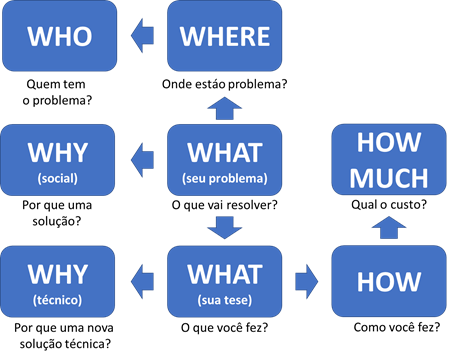
\includegraphics[width=0.7\linewidth]{Images/5w2h}
    \caption{Perguntas que devem ser respondidas antes de iniciar uma tese. Fonte: do autor.}
    \label{fig:5w2h2}
\end{figure}


\section{Quanto as figuras}

As figuras ilustrativas de todos os trabalhos dos alunos devem ser feitas, sempre que isso for possível, em linguagens gráficas da computação. A língua franca da computação atual é UML, que possui uma quantidade muito grande de diagramas que ainda podem ser especializados por meio de estereótipos.

% TODO: \usepackage{graphicx} required
\begin{figure}[hbt]
    \centering
    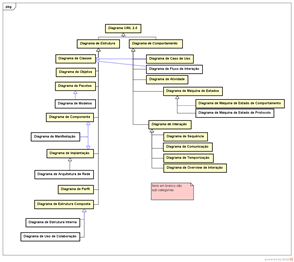
\includegraphics[width=0.7\linewidth]{Images/diagramasuml}
    \caption{Diagramas UML. Fonte: OMG}
    \label{fig:diagramasuml}
\end{figure}


Além dos diagramas de UML, que cobrem quase todos os casos possíveis, outros diagramas também são aceitáveis, como BPMN, Entidades e Relacionamentos e os da família ARIS.

Não use fluxogramas ou caixas genéricas. Fluxogramas não são mais uma linguagem usada em Computação. Diagramas têm que ter significado e é isso que as linguagens padronizadas permitem, ao contrário de caixas genéricas.

\chapter{O Prazo}

Como todo projeto, uma dissertação ou tese tem que ter um fim.

A COPPE limite o prazo de uma \textbf{dissertação em 3 anos}, mais meio ano de uma possível extensão que, pelo regulamento, não será dada facilmente.

O exame de \textbf{qualificação de mestrado} tem prazo de \textbf{dois anos sem extensão possível}.

O limite de uma \textbf{tese é de 5 anos}, com possível \textbf{extensão} (que novamente provavelmente não será dada) \textbf{de 1 ano}, com \textbf{o exame de qualificação tendo prazo de 3 anos, sem extensão possível}.

Você deve tentar atingir não os prazos máximos da COPPE, mas sim os prazos das bolas: mestrado 2 anos, doutorado 4 anos.

Sabemos que esses prazos são pequenos e eu sugiro que no máximo se chegue a 2,5 anos e 4,5 anos.

O que acontece se você usa o prazo máximo?

Vamos esquecer, momentaneamente, que você pode PERDER O PRAZO, o que é perder o trabalho de anos. Quais os outros problemas?

Primeiro, o texto sai muito pior do que devia, os experimentos são terminados de forma açodada. A banca vai reclamar muito e provavelmente reprovar com restrições e te dar um dever de casa.

Segundo, a capacidade do orientador ajudar em algo nesses casos (fim do seu prazo) é muito reduzida. Por quê? Porque seu orientador tem outras coisas para fazer no trabalho e uma vida pessoal\footnote{Aconteceu comigo, tive uma doença grave junto com o prazo final de muito alunos, incluindo 6 meses de licença, 50  dias de hospital e uma cirurgia de coração aberto. Conseguimos resolver o problema de todos, mas não foi uma boa experiência para ninguém. } , que inclui outros orientados provavelmente também fazendo a mesma coisa. Isso significa que ele, em especial eu, não vai poder realmente orientar o seu final de tese, o que é muito ruim, mas é o que acontece na prática.

Não é razoável você esperar que depois de ficar 5(3) anos fazendo seu trabalho sem muito interesse, no último instante queira uma dedicação emergencial do seu orientador. Ele estava lá por muito tempo. Pode ser que, algumas vezes, ele consiga essa dedicação, mas também pode ser que não.

Ou seja, o seu risco, como orientado, aluno e candidato ao título cresce quando o prazo está chegando. Cuidado!

\chapter{O Caderno de Pesquisa}

Uma prática que dá muito certo é os alunos manterem um caderno normal, de papel mesmo, como registro de trabalho e reuniões.

Tenha sempre o caderno ao conversar com o orientador.

Anote no caderno tudo que você fez, tudo que vai fazer.

Sei que muitos pensam em fazer isso digitalmente. Não é prático, pois não pode desenhar ou rabiscar no celular com a facilidade que faz no caderno.

Cadernos de pesquisa (ou de laboratório) são uma prática antiga que funciona. Recomendo fortemente.

Também são ótimos para criatividade e para guardar ideias que saem do nada.

Eu gosto de usar cadernos de folha branca ou quadriculada.

22	Alguns sites

\begin{outline}
\1	\url{http://www.phdcomics.com}
\2	Quadrinhos sobre doutorandos nos EUA, sou grande fã dessas tirinhas
\1	\url{http://www.dissertationdoctor.com/index.html}
\2	Apoio a doutorandos
\1	\url{http://www.phinished.org/}
\end{outline}


	\chapter{Piadas de Orientados e Orientadores}

Lembrem que toda piada tem um grau de verdade

\section{O Gênio }

Três sujeitos caminhando lado a lado, na hora do almoço. O orientador, o Bolsista de pós-graduação e o Bolsista de Graduação.

De repente, eles veem uma lâmpada velha, dessas bem antigas, das MIL e UMA Noites. O orientador pega a tal lâmpada e dá uma esfregadinha com a mão...

Logo aparece uma fumaceira e sai um Gênio, daqueles grandes, logo dizendo.... ``Normalmente eu concedo UM desejo, mas já que vocês são três, um para cada um''...

O bolsista de graduação gritou... ``Primeiro eu, primeiro eu !''

--- OK! -- disse o gênio

--- Gênio, quero ir para as Bahamas, ficar por lá com muitas mulheres colocando uvas na minha boca, à beira da piscina do melhor hotel que tiver por lá e sem nenhum tipo de preocupação monetária ou de saúde.

BUUM ! O cara desapareceu.

--- Agora eu! -- gritou o bolsista de pós-graduação

--- Pode falar -- disse o GÊNIO.

--- Seu Gênio, me manda para Honolulu. Quero duas gatas dessas bem gostosas para me acompanhar, ficar fazendo surf o ano inteiro.

BUUM! Lá foi o cara embora para os Mares do Sul.

Então o Gênio falou para o orientador: ``Agora você !''

E este diz:

--- Quero esses dois de volta no laboratório depois do almoço.

Moral da história:

Deixem o orientador sempre falar primeiro.

\section{A Tese do Coelho}

Num dia lindo e ensolarado, o coelho saiu de sua toca com o notebook e pôs-se a trabalhar, bem concentrado. Pouco depois, passou por ali a raposa e viu aquele suculento coelhinho, tão distraído, que chegou a salivar. No entanto, ela ficou intrigada com a atividade do coelho e aproximou-se, curiosa:

--- Coelhinho, o que você está fazendo aí tão concentrado?

--- Estou redigindo a minha tese de doutorado -- disse o coelho sem tirar os olhos do trabalho.

--- Humm .. . e qual é o tema da sua tese?

--- Ah, é uma teoria provando que os coelhos são os verdadeiros predadores naturais de animais como as raposas.

A raposa fica indignada:

--- Ora! Isso é ridículo! Nós é que somos os predadores dos coelhos!

--- Absolutamente! Venha comigo à minha toca que eu mostro a minha prova experimental.

O coelho e a raposa entram na toca. Poucos instantes depois ouvem-se alguns ruídos indecifráveis, alguns poucos grunhidos e depois silêncio. Em seguida o coelho volta, sozinho, e mais uma vez retoma os trabalhos da sua tese, como se nada tivesse acontecido. Meia hora depois passa um lobo. Ao ver o apetitoso coelhinho tão distraído, agradece mentalmente à cadeia alimentar por estar com o seu jantar garantido. No entanto, o lobo também acha muito curioso um coelho trabalhando naquela concentração toda. O lobo então resolve saber do que se trata aquilo tudo, antes de devorar o coelhinho:

--- Olá, jovem coelhinho. O que o faz trabalhar tão arduamente?

--- Minha tese de doutorado, seu lobo. É uma teoria que venho desenvolvendo há algum tempo e que prova que nós, coelhos, somos os grandes predadores naturais de vários animais carnívoros, inclusive dos lobos.

O lobo não se contém e cai na gargalhada com a petulância do coelho.

--- Apetitoso coelhinho! Isto é um despropósito. Nós, os lobos, é que somos os genuínos predadores naturais dos coelhos. Aliás, chega de conversa...

--- Desculpe-me, mas se você quiser eu posso apresentar a minha prova. Você gostaria de me acompanhar à minha toca?

O lobo não consegue acreditar na sua boa sorte. Ambos desaparecem toca adentro. Alguns instantes depois se ouvem uivos desesperados, ruídos de mastigação e ... silêncio. Mais uma vez o coelho retorna sozinho, impassível, e volta ao trabalho de redação da sua tese, como se nada tivesse acontecido... Dentro da toca do coelho vê-se uma enorme pilha de ossos ensanguentados e pelancas de diversas ex-raposas e, ao lado desta, outra pilha ainda maior de ossos e restos mortais daquilo que um dia foram lobos. Ao centro das duas pilhas de ossos, um enorme LEÃO, satisfeito, bem alimentado e sonolento, a palitar os dentes.

MORAL DA HISTORIA:

\begin{itemize}
\item Não importa quão absurdo é o tema de sua tese.
\item Não importa se você não tem o mínimo fundamento científico.
\item Não importa se os seus experimentos nunca cheguem a provar sua teoria.
\item Não importa nem mesmo se suas idéias vão contra o mais óbvio dos conceitos lógicos...
\item o que importa é quem é seu orientador...
\end{itemize}

\section{Ditados}
\begin{itemize}
\item	"Tudo que é simples dá mais trabalho que merece"
\item	"Se é estúpido, mas funciona, então não é tão estúpido assim."
\item	"Escopo bom é escopo pequeno"
\item	"Metodologia é função do problema e não o contrário"
\item	"Banca boa é banca de amigos"
\item	"Bibliografia tem de incluir tanto clássicos quanto textos recentes"
\item	"Ciência é Marketing, "venda" sua tese para a banca"
\item	"Cuidado para não misturar autores incompatíveis"
\item	"Planeje seus experimentos antes de colher os dados, senão você pode não ser capaz de analisá-los."
\item	"All models are wrong, but some are useful". - George E. P. Box
\item	"Be regular and orderly in your life so that you may be violent and original in your work" - Flaubert
\item	"Computer Science is no more about computers than astronomy is about telescopes." – Edsger Dijkstra
\item	"Truth is what stands the test of experience." - Albert Einstein
\item	"The more we know, the more we feel our ignorance; the more we feel how much remains unknown"– Sir Humphry Davy
\item	"Science may be described as the art of systematic oversimplification." –  Karl Popper
\item	"The great tragedy of Science – - the slaying of a beautiful hypothesis by an ugly fact." –  Thomas Henry Huxley
\item	"The story of a theory's failure often strikes readers as sad and unsatisfying. Since science thrives on self-correction, we who practice this most challenging of human arts do not share such a feeling. We may be unhappy if a favored hypothesis loses or chagrined if theories that we proposed prove inadequate. But refutation almost always contains positive lessons that overwhelm disappointment, even when [...] no new and comprehensive theory has yet filled the void." –  Stephen Jay Gould (1941-2002), "Bully for Brontosaurus", The Face of Miranda (1991)
\item	"There must be no barriers for freedom of inquiry. There is no place for dogma in science. The scientist is free, and must be free to ask any question, to doubt any assertion, to seek for any evidence, to correct any errors." - Robert Oppenheimer
\item	"To know that we know what we know, and to know that we do not know what we do not know, that is true knowledge." - Copernicus
\item	"I believe there is no philosophical high-road in science, with epistemological signposts. No, we are in a jungle and find our way by trial and error, building our road behind us as we proceed." - Max Born
\item	"Nothing in this world is to be feared... only understood." - Marie Curie
\item	"The fact that some geniuses were laughed at does not imply that all who are laughed at are geniuses. They laughed at Columbus, they laughed at Fulton, they laughed at the Wright brothers. But they also laughed at Bozo the Clown." - Carl Sagan
\item	“A scientist is happy, not in resting on his attainments but in the steady acquisition of fresh knowledge." - Max Planck
\item	"It doesn't matter how beautiful your theory is, it doesn't matter how smart you are. If it doesn't agree with experiment, it's wrong" - Richard Feynman
\item	Crash programs fail because they are based on theory that, with nine women pregnant, you can get a baby a month - Wernher von Braun.
\item	Early to bed, early to rise, work like hell and advertise- Wernher von Braun.
\item	One test result is worth one thousand expert opinions- Wernher von Braun.
\item	Science does not have a moral dimension. It is like a knife. If you give it to a surgeon or a murderer, each will use it differently- Wernher von Braun.
\item	The universe is hostile only when you do not know its laws. To those who know and obey, the universe is friendly- Wernher von Braun.
\item	With every new answer unfolded, science has consistently discovered at least three new questions- Wernher von Braun.
\end{itemize}


\chapter{Mensagem a Garcia}

Um texto final para motivar os orientados.

Mensagem a Garcia Elbert Hubbard – fevereiro de 1899

Em todo este caso cubano, um homem se destaca no horizonte de minha memória. Quando irrompeu a guerra entre a Espanha e os Estados Unidos, o que importava aos americanos era comunicar-se, rapidamente, com o chefe dos revoltosos – chamado Garcia - que se encontrava em uma fortaleza desconhecida, no interior do sertão cubano. Era impossível um entendimento com ele pelo correio ou pelo telégrafo. No entanto, o Presidente precisava de sua colaboração, e isso o quanto antes. Que fazer? Alguém lembrou: ``Há um homem chamado Rowan... e se alguma pessoa é capaz de encontrar Garcia, esta pessoa é Rowan''.

Rowan foi trazido à presença do Presidente, que lhe confiou uma carta com a incumbência de entregá-la a Garcia. Não vêm ao caso narrar aqui como esse homem tomou a carta, guardou-a num invólucro impermeável, amarrou a ao peito e, após quatro dias, saltou de um pequeno barco, alta noite, nas costas de Cuba; ou como se embrenhou no sertão para, depois de três semanas, surgir do outro lado da ilha, tendo atravessado a pé um país hostil, e entregue a carta a Garcia. O ponto que desejo frisar é este: Mac Kinley deu a Rowan uma carta destinada a Garcia; Rowan tomou-a e nem sequer perguntou: ``Onde é que ele está?''.

Eis aí um homem cujo busto merecia ser fundido em bronze e sua estátua colocada em cada escola. Não é só de sabedoria que a juventude precisa... Nem de instruções sobre isto ou aquilo. Precisa, sim, de um endurecimento das vértebras para poder mostrar-se altiva no exercício de um cargo; para atuar com diligência; para dar conta do recado; para, em suma, levar uma mensagem a Garcia. O General Garcia já não é deste mundo, mas há outros Garcias. A nenhum homem que se tenha empenhado em levar adiante uma tarefa em que a ajuda de muitos se torne precisa tem sido poupados momentos de verdadeiro desespero ante a passividade de grande número de pessoas ante a inabilidade ou falta de disposição de concentrar a mente numa determinada tarefa... e fazê-la. A regra geral é: assistência regular, desatenção tola, indiferença irritante e trabalho malfeito.

Ninguém pode ser verdadeiramente bem-sucedido, exceto se lançar mão de todos os meios ao seu alcance, para obrigar outras pessoas a ajudá-lo, a não ser que Deus Onipotente, na sua grande misericórdia, faça um milagre enviando-lhe, como auxiliar, um anjo de luz. Leitor amigo, tu mesmo podes tirar a prova. Está sentado no teu escritório, rodeado de meia dúzia de empregados. Pois bem, chama um deles e pede-lhe: ``Queria ter a bondade de consultar a enciclopédia e de fazer a descrição resumida da vida de Corrégio''.

Dar-se-á o caso de o empregado dizer, calmamente: –  ``Sim, senhor'' e executar o que lhe pediste? Nada disso! Olhar-te-á admirado para fazer uma ou algumas das seguintes perguntas:

---  Quem é Corrégio?

---  Que enciclopédia?

---  Onde está a enciclopédia?

---  Fui contratado para fazer isso?

--- E se Carlos o fizesse?

---  Esse sujeito já morreu?

--–  Precisa disso com urgência?

--–  Não seria melhor eu trazer o livro para o Senhor procurar?

–-- Para que quer saber isso?

Eu aposto dez contra um que, depois de haveres respondido a tais perguntas e explicado a maneira de procurar os dados pedidos, e a razão por que deles precisas, teu empregado irá pedir a um companheiro que o ajude a encontrar Corrégio e depois voltará para te dizer que tal homem nunca existiu. Evidentemente pode ser que eu perca a aposta, mas, seguindo uma regra geral, jogo na certa. Ora, se fores prudente, não te darás ao trabalho de explicar ao teu "ajudante" que Corrégio se escreve com ``C'' e não com ``K'', mas limitar-te-á a dizer calmamente, esboçando o melhor sorriso: ``Não faz mal... não se incomode''. É essa dificuldade de atuar independentemente, essa fraqueza de vontade, essa falta de disposição de, solicitamente, se por em campo e agir, é isso o que impede o avanço da humanidade, fazendo-o recuar para um futuro bastante remoto. Se os homens não tomam a iniciativa de agir em seu próprio proveito, que farão se o resultado de seu esforço resultar em benefício de todos? Por enquanto parece que os homens ainda precisam ser dirigidos.

O que mantém muitos empregados no seu posto e o faz trabalhar é o medo de, se não o fizer, ser despedido ou transferido no fim do mês. Anuncia-se precisar de um taquígrafo e nove entre dez candidatos à vaga não saberão ortografar nem pontuar, e –  o que é pior – pensa não ser necessário sabê-lo.

``Olhe aquele funcionário'' -–  dizia o chefe de uma grande fábrica. É um excelente funcionário. Contudo, se eu lhe perguntasse por que seu trabalho é necessário ou por que é feito dessa maneira e não de outra, ele seria incapaz de me responder. Nunca deve ter pensado nisso. Faz apenas aquilo que lhe ensinaram, há mais de 3 anos, e nem um pouco a mais".

``Será possível confiar-se a tal homem uma carta para entregá-la a Garcia?''.

Conheço um homem de aptidões realmente brilhantes, mas sem a fibra necessária para dirigir um negócio próprio e que ainda se torna completamente nulo para qualquer outra pessoa devido à suspeita que constantemente abriga de que seu patrão o esteja oprimindo ou tencione oprimi-lo. Sem poder mandar, não tolera que alguém o mande. Se lhe fosse confiada a mensagem a Garcia retrucaria, provavelmente:

--–  Leve-a você mesmo!.

Hoje esse homem perambula errante, pelas ruas em busca de trabalho, em estado quase de miséria. No entanto, ninguém se aventura a dar-lhe trabalho porque é uma personificação do descontentamento e do espírito da discórdia. Não aceitando qualquer conselho ou advertência, a única coisa capaz de nele produzir algum efeito seria um bom pontapé dado com a ponta de uma bota 44, sola grossa e bico largo.

Pautemos nossa conduta por aqueles homens, dirigente ou dirigida, que realmente se esforçam por realizar o seu trabalho. Aqueles cujos cabelos ficam mais cedo envelhecidos na incessante luta que estão desempenhando contra a indiferença e a ingratidão, justamente daqueles que, sem o seu espírito empreendedor, andariam famintos e sem lar.

Estarei pintando o quadro com cores por demais escuras?

Não há excelência na nobreza de si mesmo; farrapos não servem de recomendação. Nem todos os ricos são gananciosos e tiranos, da mesma forma que nem todos os pobres são virtuosos. Todas as minhas simpatias pertencem ao homem que trabalha, fazendo o que deve ser feito, melhorando o que pode ser melhorado, ajudando sem exigir ajuda. É o homem que, ao lhe ser confiada uma carta para Garcia, toma a missiva e, sem a intenção de jogá-la na primeira sarjeta, entrega-a ao destinatário. Esse homem nunca ficará "encostado", nem pedirá que lhe façam favores.

A civilização busca ansiosamente, insistentemente, homens nessa condição. Tudo que tal homem pedir, se lhe há de conceder. Precisa-se dele em cada vila, em cada lugarejo, em cada escritório, em cada oficina, em cada loja, fábrica ou venda. O grito do mundo inteiro praticamente se resume nisso:

\gxatencao{PRECISA-SE –  E PRECISA-SE COM URGÊNCIA –  DE UM HOMEM CAPAZ DE LEVAR UMA MENSAGEM A GARCIA.}




\printindex

\printbibliography
%\bibliography{citados.bib}
\appendix


\backmatter

\end{document}
